%%===========================================================%%
%%                                                           %%
%%                   SYSTEMATIC ERRORS                       %%
%%                                                           %%
%%===========================================================%%


\chapter{Systematic errors}\label{chap:systematicErrors}
\section{TPC track reconstruction efficiency}\label{sec:tpcSystematics}
\subsection{Embedding (pile-up) effect}\label{subsec:TpcEffSystPileUp}
One major difference between simulation and real data is the presence of pile-up
events. The average number of pile-up tracks in
a triggering event is proportional to the BBC coincidence rate. It is expected that
the difference between simulation and real data drops at lower BBC rates, and the
effects of pile-up tracks could be much reduced by fitting the tracking efficiency as a
function of BBC rate and using the extrapolated value at zero luminosity to compare
with simulation.\newline

%---------------------------
\begin{wrapfigure}{r}{0.45\textwidth}\vspace*{-9pt}
	\centering
	\includegraphics[width=0.45\textwidth, page=5]{graphics/systematicsEfficiency/bbc_and/Out.pdf}
	\caption[Number of events in embedded MC as a function of BBC\_AND rate.]
	{Number of events in embedded MC as a function of BBC\_AND rate. The black and red lines represent the events with \mbox{$<\text{BBC\_AND}>=700$~kHz} and \mbox{$<\text{BBC\_AND}>=1400$~kHz},  respectively.}
	\label{fig:events_bbc_and}%\vspace*{-29pt}
\end{wrapfigure}
%---------------------------
\noindent The embedded MC was divided into two samples due to mean BBC\_AND rate: \mbox{$<\text{BBC\_AND}>=700$~kHz} and \mbox{$<\text{BBC\_AND}>=1400$~kHz}. Next, the track reconstruction efficiency was calculated for those two samples and no-pile-up MC corresponding to them. The difference between TPC track reconstruction efficiences for pile-up and no-pile-up MCs was calculated as:
\begin{equation}
	\Delta\epsilon_{ TPC}^{1400/700\text{ kHz}} = \frac{N_{reco}^{no-pile-up}-N_{reco}^{pile-up}}{N_{gen}}\\
	\label{eq:tpcSyst}
\end{equation}
where:\\
$N_{gen}$-number of MC tracks,\\
$N_{reco}^{no-pile-up}$ - number of reconstructed tracks, matched with MC tracks in no-pile-up MC,\\
$N_{reco}^{pile-up}$ - number of reconstructed tracks, matched with MC tracks in pile-up MC.

The difference between high and low pile-up runs is given by:
\begin{equation}
\Delta\epsilon_{ TPC} =\Delta\epsilon_{ TPC}^{1400\text{ kHz}}-2\cdot\Delta\epsilon_{ TPC}^{700\text{ kHz}}
\label{eq:tpcSystDifference}
\end{equation}
Finally, above difference, shown in  \Cref{fig:systError1Dtpc,fig:systError2Dtpc} for $\pi^\pm$, varies between $2-3\%$ and was taken as systematic uncertainty related to TPC track reconstruction efficiency.
%\vspace{10em}
\begin{figure}[hb]
	\centering
	\parbox{0.495\textwidth}{
		\centering
		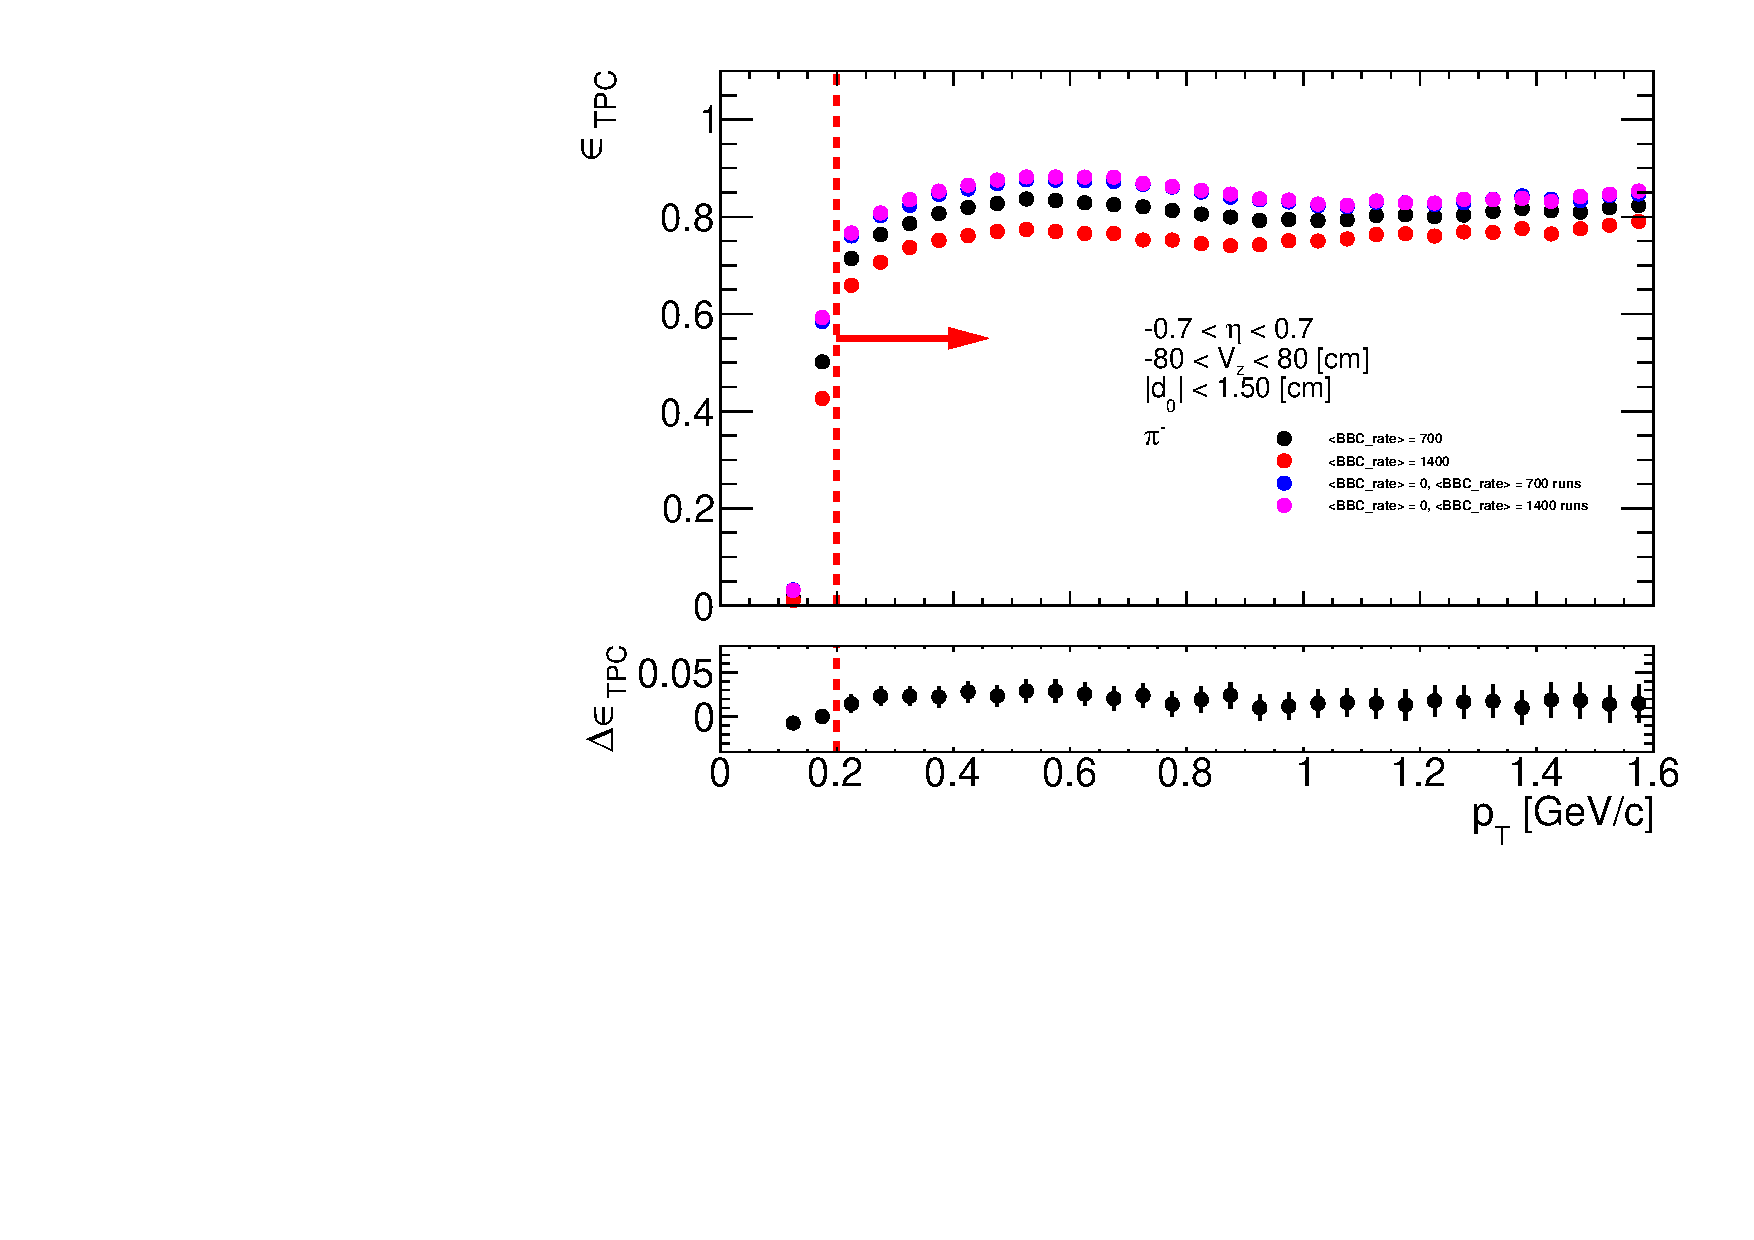
\includegraphics[width=\linewidth,page=1]{graphics/systematicsEfficiency/bbc_and/tpcEffi_d0_1_5_etapt_1.pdf}\\
	}~
	\parbox{0.495\textwidth}{
		\centering
		\includegraphics[width=\linewidth,page=2]{graphics/systematicsEfficiency/bbc_and/tpcEffi_d0_1_5_etapt_1.pdf}\\
	}%
	\caption[$\pi^\pm$ TPC track reconstruction efficiency as a function of $p_T$ $\left(|\eta|<0.7, |V_z|<80\text{ cm}\right)$ for embedded MC samples with \mbox{$<\text{BBC\_AND}>=700$~kHz} and \mbox{$<\text{BBC\_AND}>=1400$~kHz}]{$\pi^\pm$ TPC track reconstruction efficiency as a function of $p_T$ $\left(|\eta|<0.7, |V_z|<80\text{ cm}\right)$ for embedded MC samples with \mbox{$<\text{BBC\_AND}>=700$~kHz} and \mbox{$<\text{BBC\_AND}>=1400$~kHz}. The efficiences from corresponding no-pile-up MC samples were also shown. Additionally, the differences  from Eq. \ref{eq:tpcSystDifference} were drawn in the bottom of each plot.}
	\label{fig:systError1Dtpc}
\end{figure}
\begin{figure}[H]
	\centering
	\parbox{0.495\textwidth}{
		\centering
		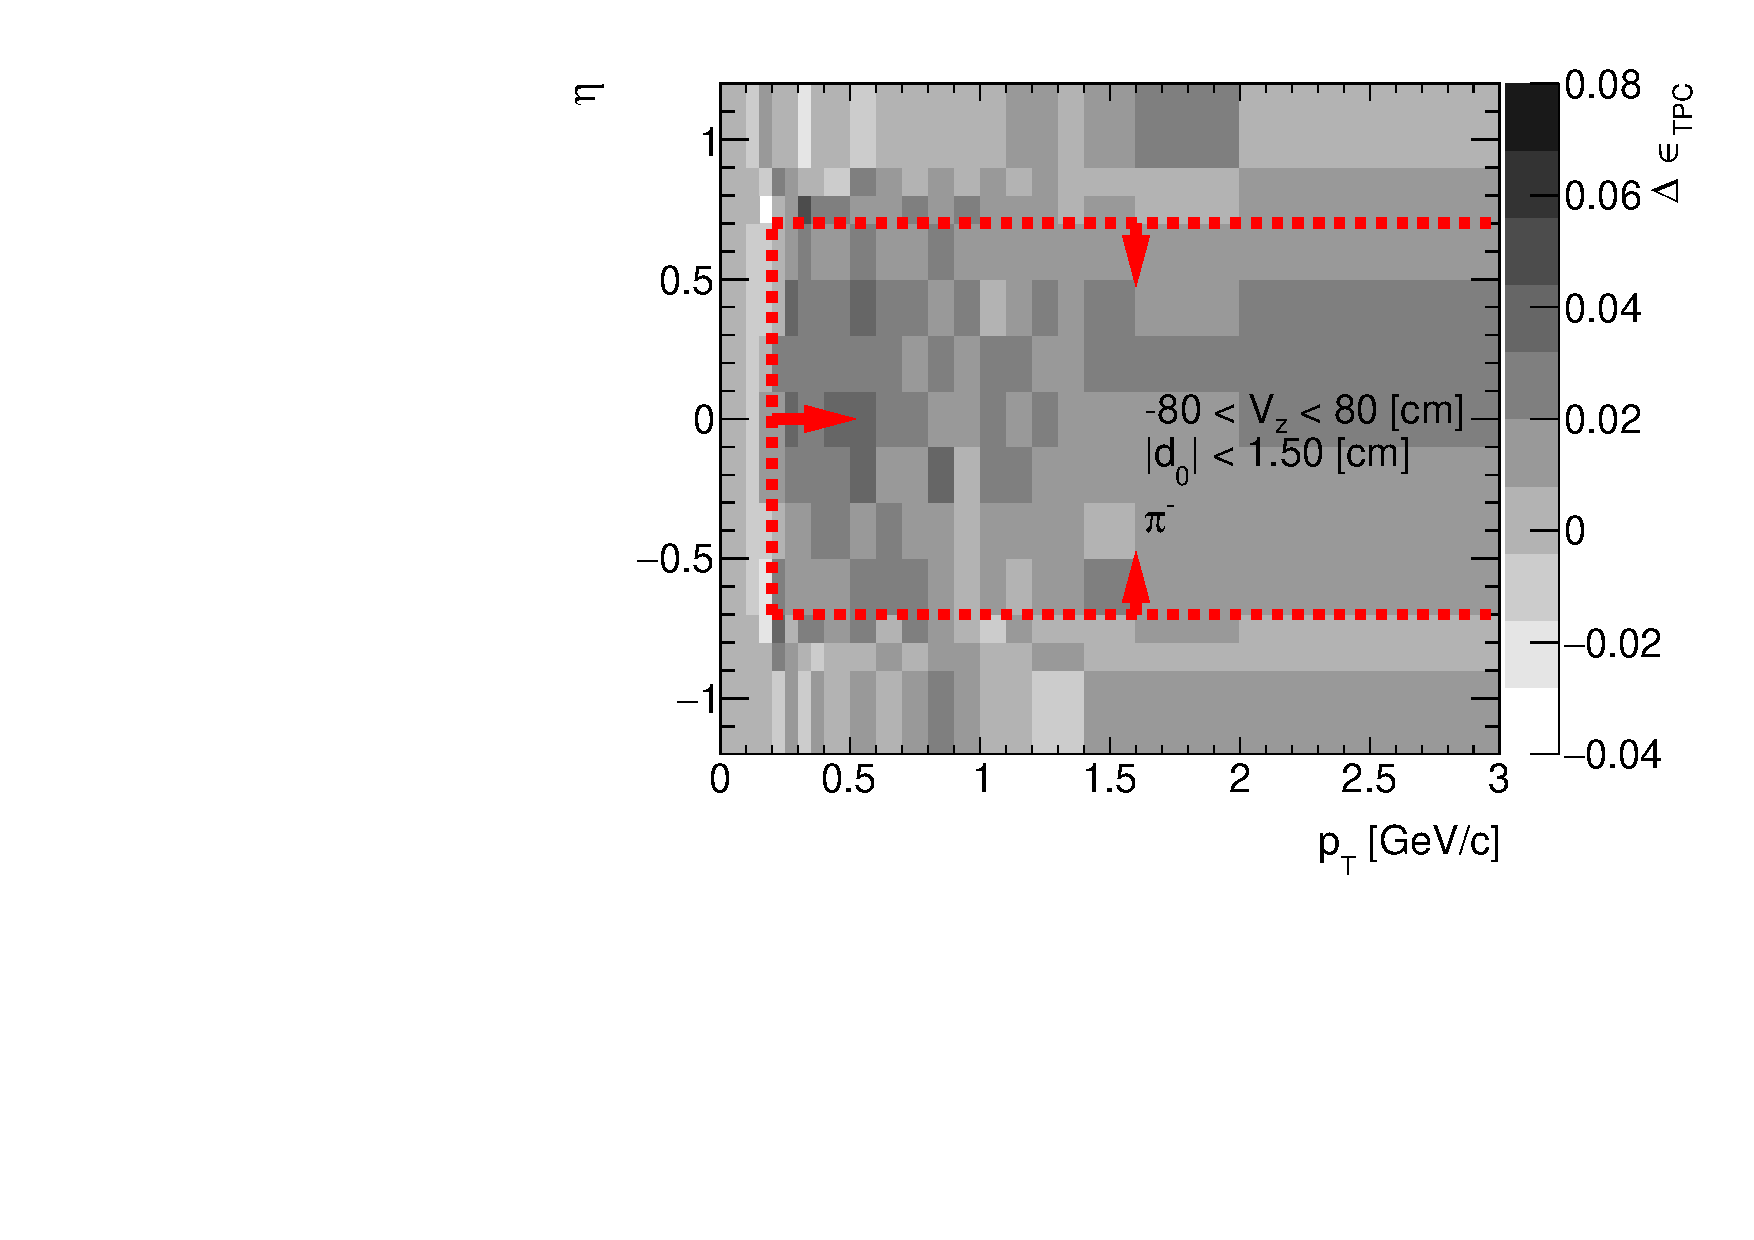
\includegraphics[width=\linewidth,page=1]{graphics/systematicsEfficiency/bbc_and/tpcEffi_d0_1_5_etapt_12D.pdf}\\
	}~
	\parbox{0.495\textwidth}{
		\centering
		\includegraphics[width=\linewidth,page=2]{graphics/systematicsEfficiency/bbc_and/tpcEffi_d0_1_5_etapt_12D.pdf}\\
	}%
	\caption[The difference $\Delta\epsilon_{ TPC} =\Delta\epsilon_{ TPC}^{1400\text{ kHz}}-2\cdot\Delta\epsilon_{ TPC}^{700\text{ kHz}}$ for $\pi^\pm$ as a function of $p_T$ and $\eta$ $\left(|V_z|<80\text{ cm}\right)$]{The difference $\Delta\epsilon_{ TPC} =\Delta\epsilon_{ TPC}^{1400\text{ kHz}}-2\cdot\Delta\epsilon_{ TPC}^{700\text{ kHz}}$ for $\pi^\pm$ as a function of $p_T$ and $\eta$ $\left(|V_z|<80\text{ cm}\right)$. }
	\label{fig:systError2Dtpc}
\end{figure}

\subsection{Dead material effect on TPC track reconstruction efficiency}\label{sec:deadMaterialSystematics}
The amount of dead material in front of TPC differs up to $25\%$ between data and simulation (see Sec.~\ref{chap:deadMaterial}). First, the~amount of lost particles, $\delta\epsilon_{ TPC}$, due to the interaction with dead material in front of TPC was estimated using  no-pile-up  MC samples. The sample result for $\pi^-$ in CD and SD is shown in Fig. \ref{fig:dead_materialCDSD3D}. The remaning plots for other $z$-vertex bins and other particles are contained  in Appendix \ref{appendix:deadMaterial}.
The symmetric systematic uncertainty to the TPC track reconstruction efficiency due to dead material was introduced as $\pm 0.25 \cdot\delta\epsilon_{ TPC}$.
In Fig. \ref{fig:dead_materialCDSD1D}  the systematic uncertainty is shown for each particle species in CD and SD as a~function of $p_T$ $\left(|\eta|<0.7, |V_{z}|<80 \text{ cm}\right)$. 

\begin{figure}[h!]%\vspace{-10pt}
	\centering
	\includegraphics[width=0.9\linewidth,page=9]{graphics/systematicsEfficiency/deadMaterial/secondaries_Unbinned_SDCD_.pdf}\vspace*{-8pt}
	\caption[The amount of lost $\pi^-$ due to the interaction with dead material in front of TPC as a function of $p_T$, $\eta$ in sample $z$-vertex bin in CD and SD]{The amount of lost $\pi^-$ due to the interaction with dead material in front of TPC. Sample plot represents the fraction of lost $\pi^-$, $\delta\epsilon_{ TPC}$ ($z$-axis), as a function of true particle pseudorapidity $\eta$ ($y$-axis) and transverse momentum $p_{T}$ ($x$-axis) in single $z$-vertex bin. Red lines and arrows indicate region accepted in the analysis.}\label{fig:dead_materialCDSD3D}
\end{figure}
\begin{figure}[hb]
\centering
\parbox{0.49\textwidth}{
  \centering
  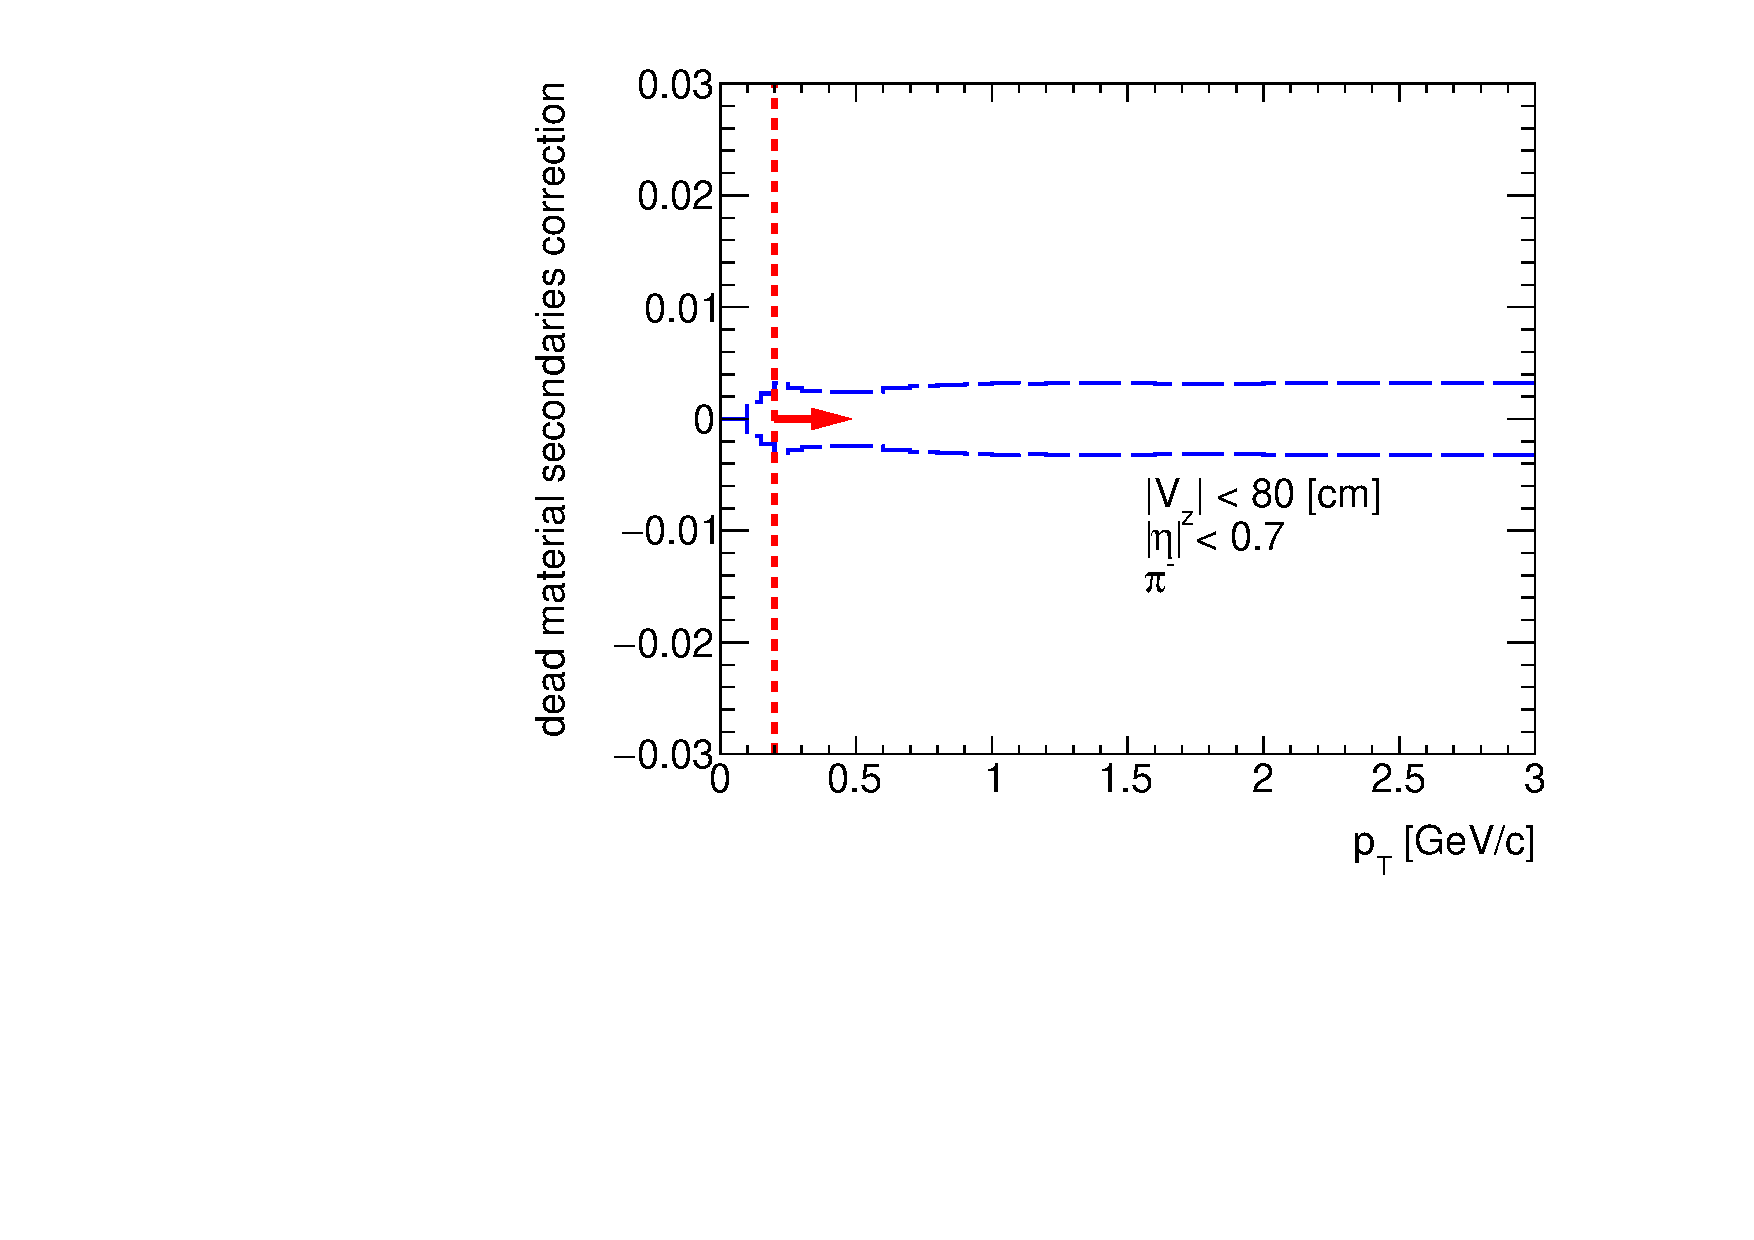
\includegraphics[width=\linewidth,page=1]{graphics/systematicsEfficiency/deadMaterial/secondaries_Unbinned_SDCD_1D.pdf}\\
  \includegraphics[width=\linewidth,page=2]{graphics/systematicsEfficiency/deadMaterial/secondaries_Unbinned_SDCD_1D.pdf}\\
  \includegraphics[width=\linewidth,page=3]{graphics/systematicsEfficiency/deadMaterial/secondaries_Unbinned_SDCD_1D.pdf}\\
  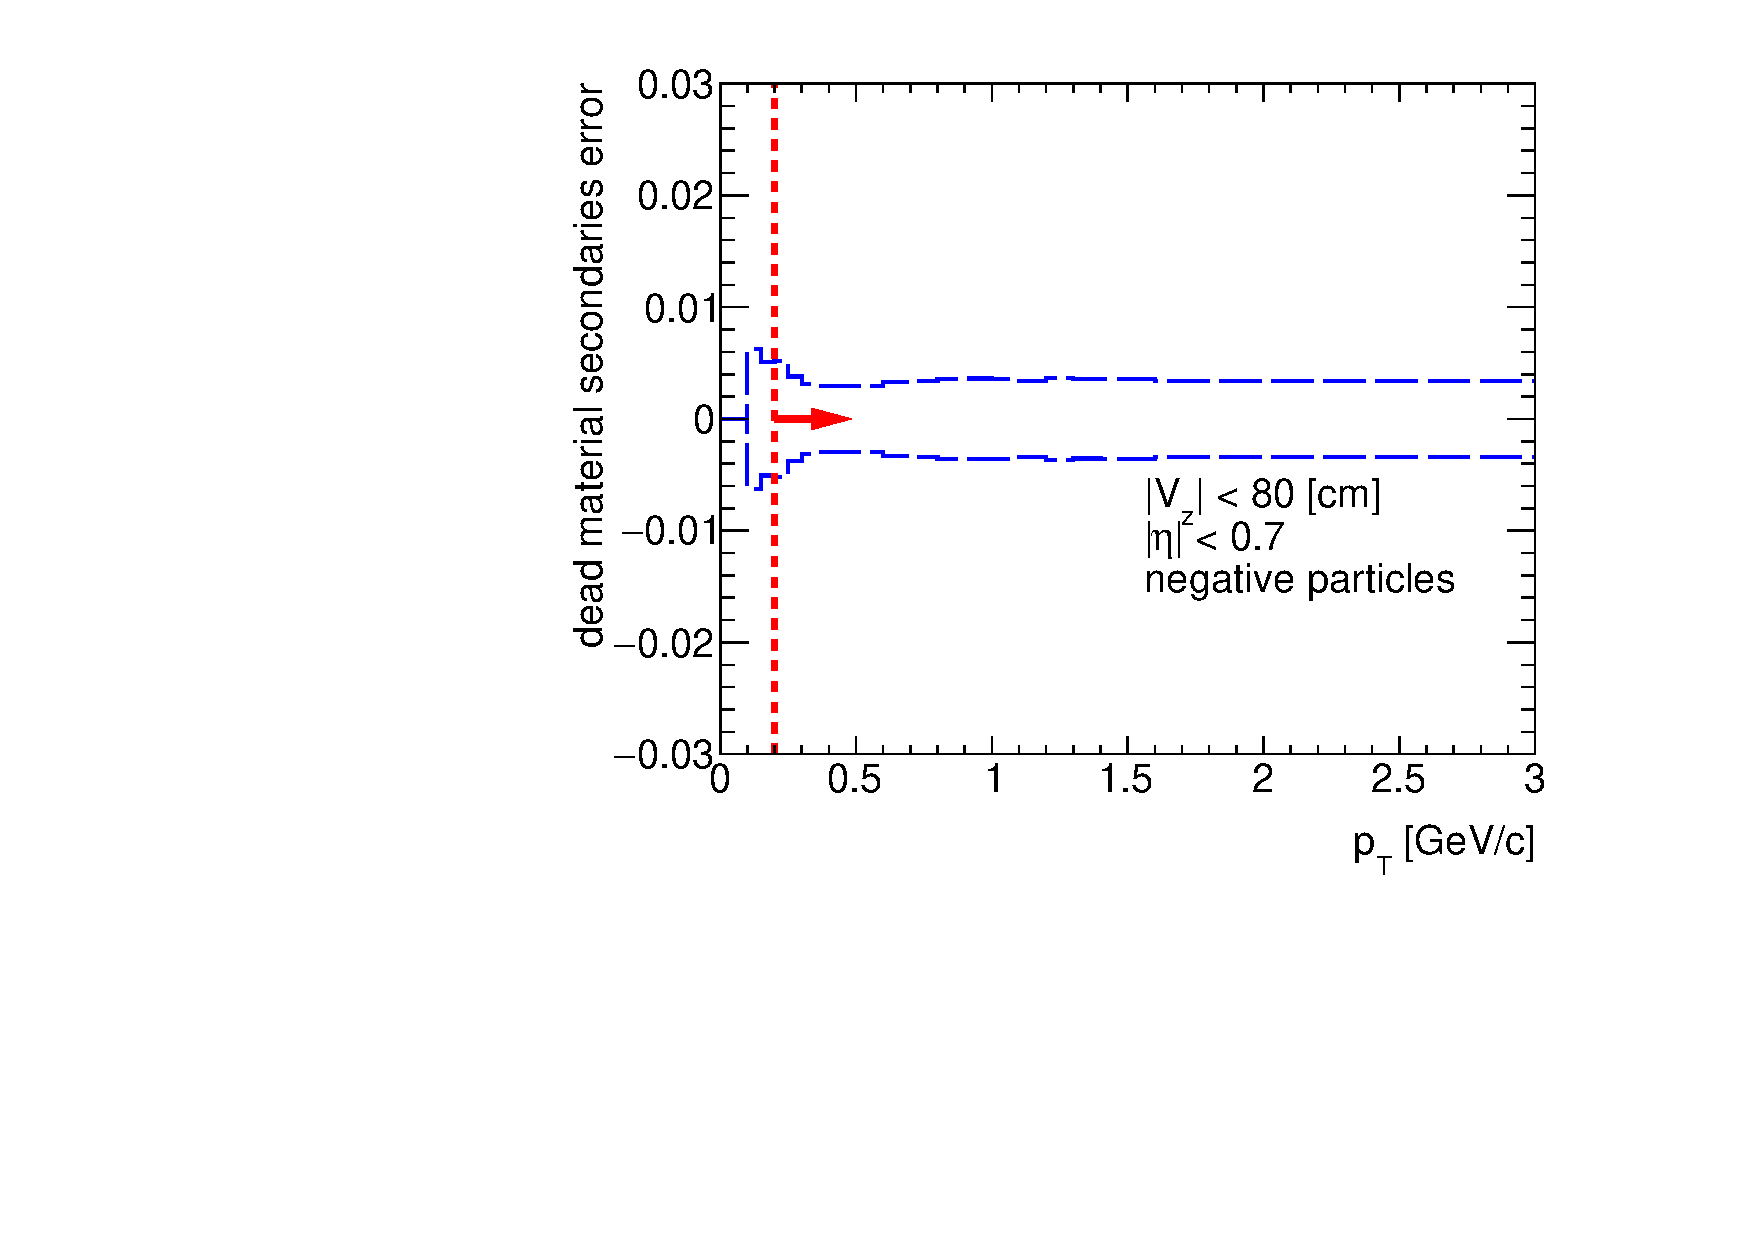
\includegraphics[width=\linewidth,page=1]{graphics/systematicsEfficiency/deadMaterial/secondaries_Unbinned_Charged_SDCD1D.pdf}\\
}~
\parbox{0.49\textwidth}{
  \centering
  \includegraphics[width=\linewidth,page=4]{graphics/systematicsEfficiency/deadMaterial/secondaries_Unbinned_SDCD_1D.pdf}\\
  \includegraphics[width=\linewidth,page=5]{graphics/systematicsEfficiency/deadMaterial/secondaries_Unbinned_SDCD_1D.pdf}\\
  \includegraphics[width=\linewidth,page=6]{graphics/systematicsEfficiency/deadMaterial/secondaries_Unbinned_SDCD_1D.pdf}\\
  \includegraphics[width=\linewidth,page=2]{graphics/systematicsEfficiency/deadMaterial/secondaries_Unbinned_Charged_SDCD1D.pdf}
}%
\caption[The systematic uncertainty to the TPC track reconstruction efficiency due to  amount of dead material in front of TPC using MC samples for CD and SD]{The systematic uncertainty to the TPC track reconstruction efficiency due to  amount of dead material in front of TPC using MC samples for CD and SD. Each plot represents the systematic uncertainty as a~function of true particle $p_T$ $\left(|\eta|<0.7, |V_{z}|<80 \text{ cm}\right)$ for given particle species: $\pi^-$,$\pi^+$, $K^-$, $K^+$, $\bar{p}$, $p$, negative and positive particles without identification. Red lines and arrows indicate region accepted in the analysis.}\label{fig:dead_materialCDSD1D}
\end{figure}



\section{TOF matching efficiency}\label{sec:tofSystematics}
\subsection{Embedding (pile-up) effect}\label{sec:tofSystematicsPileUpEffect}
The approach to calculate the systematic uncertainty on TOF matching efficiency related to pile-up was quite similar to the one used for TPC track reconstruction efficiency (Sec.~\ref{subsec:TpcEffSystPileUp}). However, the TOF matching efficiency is conditional and depends on TPC track reconstruction efficiency. Since that, the difference between high and low pile-up runs is given by:
\begin{equation}
\Delta\epsilon_{ TOF}^{1400/700\text{ kHz}}=\frac{N_{TPC-TOF}^{no-pile-up}}{N_{TPC}^{no-pile-up}}-\frac{N_{TPC-TOF}^{pile-up}}{N_{TPC}^{pile-up}}
\label{eq:tofSyst}
\end{equation}
where:\\
$N_{TPC-TOF}^{pile-up}$ - number of reconstructed tracks, matched with MC tracks and TOF hit in pile-up MC,\\
$N_{TPC-TOF}^{no-pile-up}$ - number of reconstructed tracks, matched with MC tracks and TOF hit in no-pile-up MC,\\
$N_{TPC}^{pile-up}$ - number of reconstructed tracks, matched with MC tracks in pile-up MC,\\
$N_{TPC}^{no-pile-up}$ - number of reconstructed tracks, matched with MC tracks in no-pile-up MC.

\noindent Next the difference between high and low pile-up events was calculated withe the formula similar to the one given by Eq. \ref{eq:tpcSystDifference} and is shown in \Cref{fig:systError1Dtof,fig:systError2Dtof}. The origin of  $N_{TPC-TOF}$ increase is not known (it may be due to lack of pile-up in TPC or TOF). Since that, it is impossible to correctly calculate the statistical error for $\Delta\epsilon_{ TOF}$. Nevertheless, $\Delta\epsilon_{ TOF}$ is  smaller than $0.5\%$ and can be neglected in comparison with other systematic uncertainties.
\begin{figure}[hb]
	\centering
	\parbox{0.495\textwidth}{
		\centering
		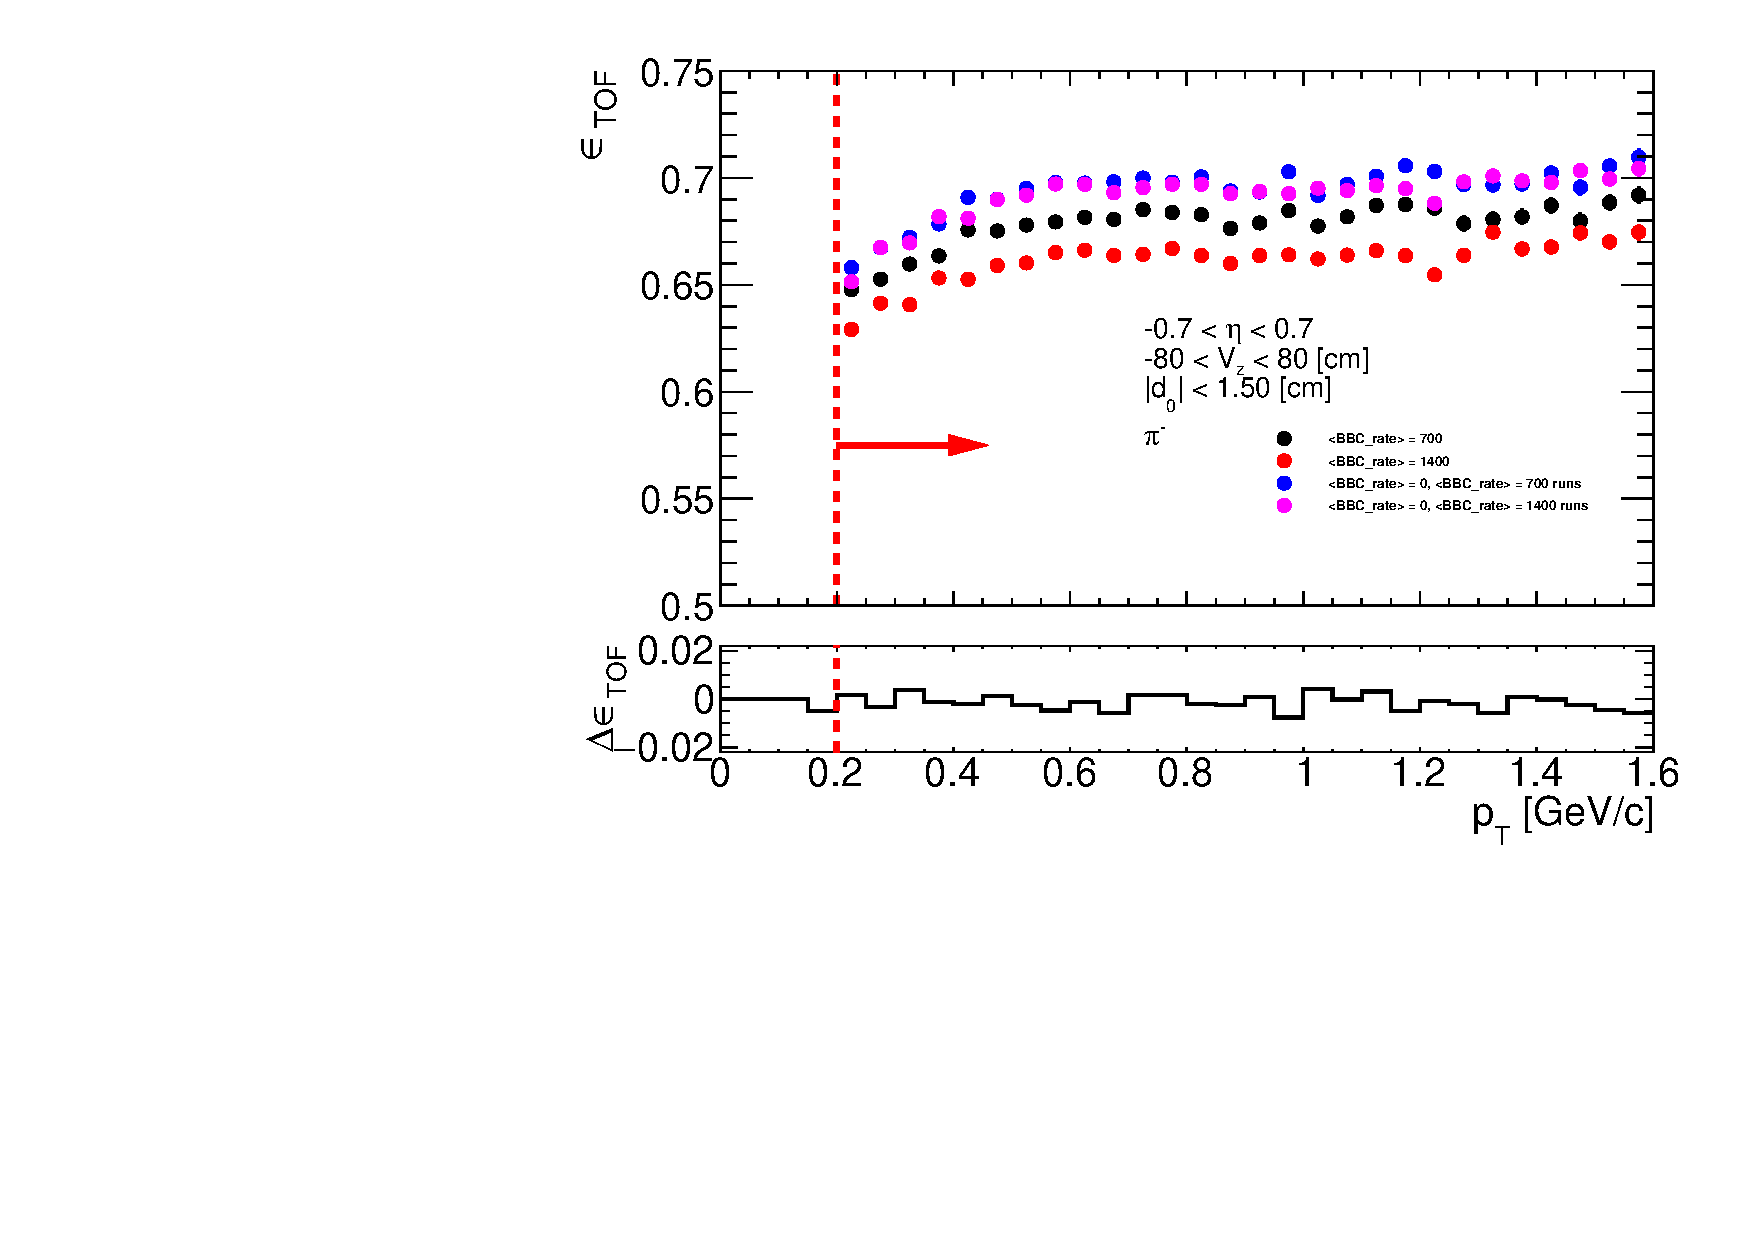
\includegraphics[width=\linewidth,page=1]{graphics/systematicsEfficiency/bbc_and/tofEffi_d0_1_5_etapt_1.pdf}\\
	}~
	\parbox{0.495\textwidth}{
		\centering
		\includegraphics[width=\linewidth,page=2]{graphics/systematicsEfficiency/bbc_and/tofEffi_d0_1_5_etapt_1.pdf}\\
	}%
	\caption[$\pi^\pm$ TOF matching efficiency as a function of $p_T$ $\left(|\eta|<0.7, |V_z|<80\text{ cm}\right)$ for embedded MC samples with \mbox{$<\text{BBC\_AND}>=700$~kHz} and \mbox{$<\text{BBC\_AND}>=1400$~kHz}]{$\pi^\pm$ TOF matching efficiency as a function of $p_T$ $\left(|\eta|<0.7, |V_z|<80\text{ cm}\right)$ for embedded MC samples with \mbox{$<\text{BBC\_AND}>=700$~kHz} and \mbox{$<\text{BBC\_AND}>=1400$~kHz}. The efficiences from corresponding no-pile-up MC samples were also shown. Additionally, the differences  from Eq. \ref{eq:tpcSystDifference} were drawn in the bottom of each plot.}
	\label{fig:systError1Dtof}
\end{figure}
\begin{figure}[H]
	\centering
	\parbox{0.495\textwidth}{
		\centering
		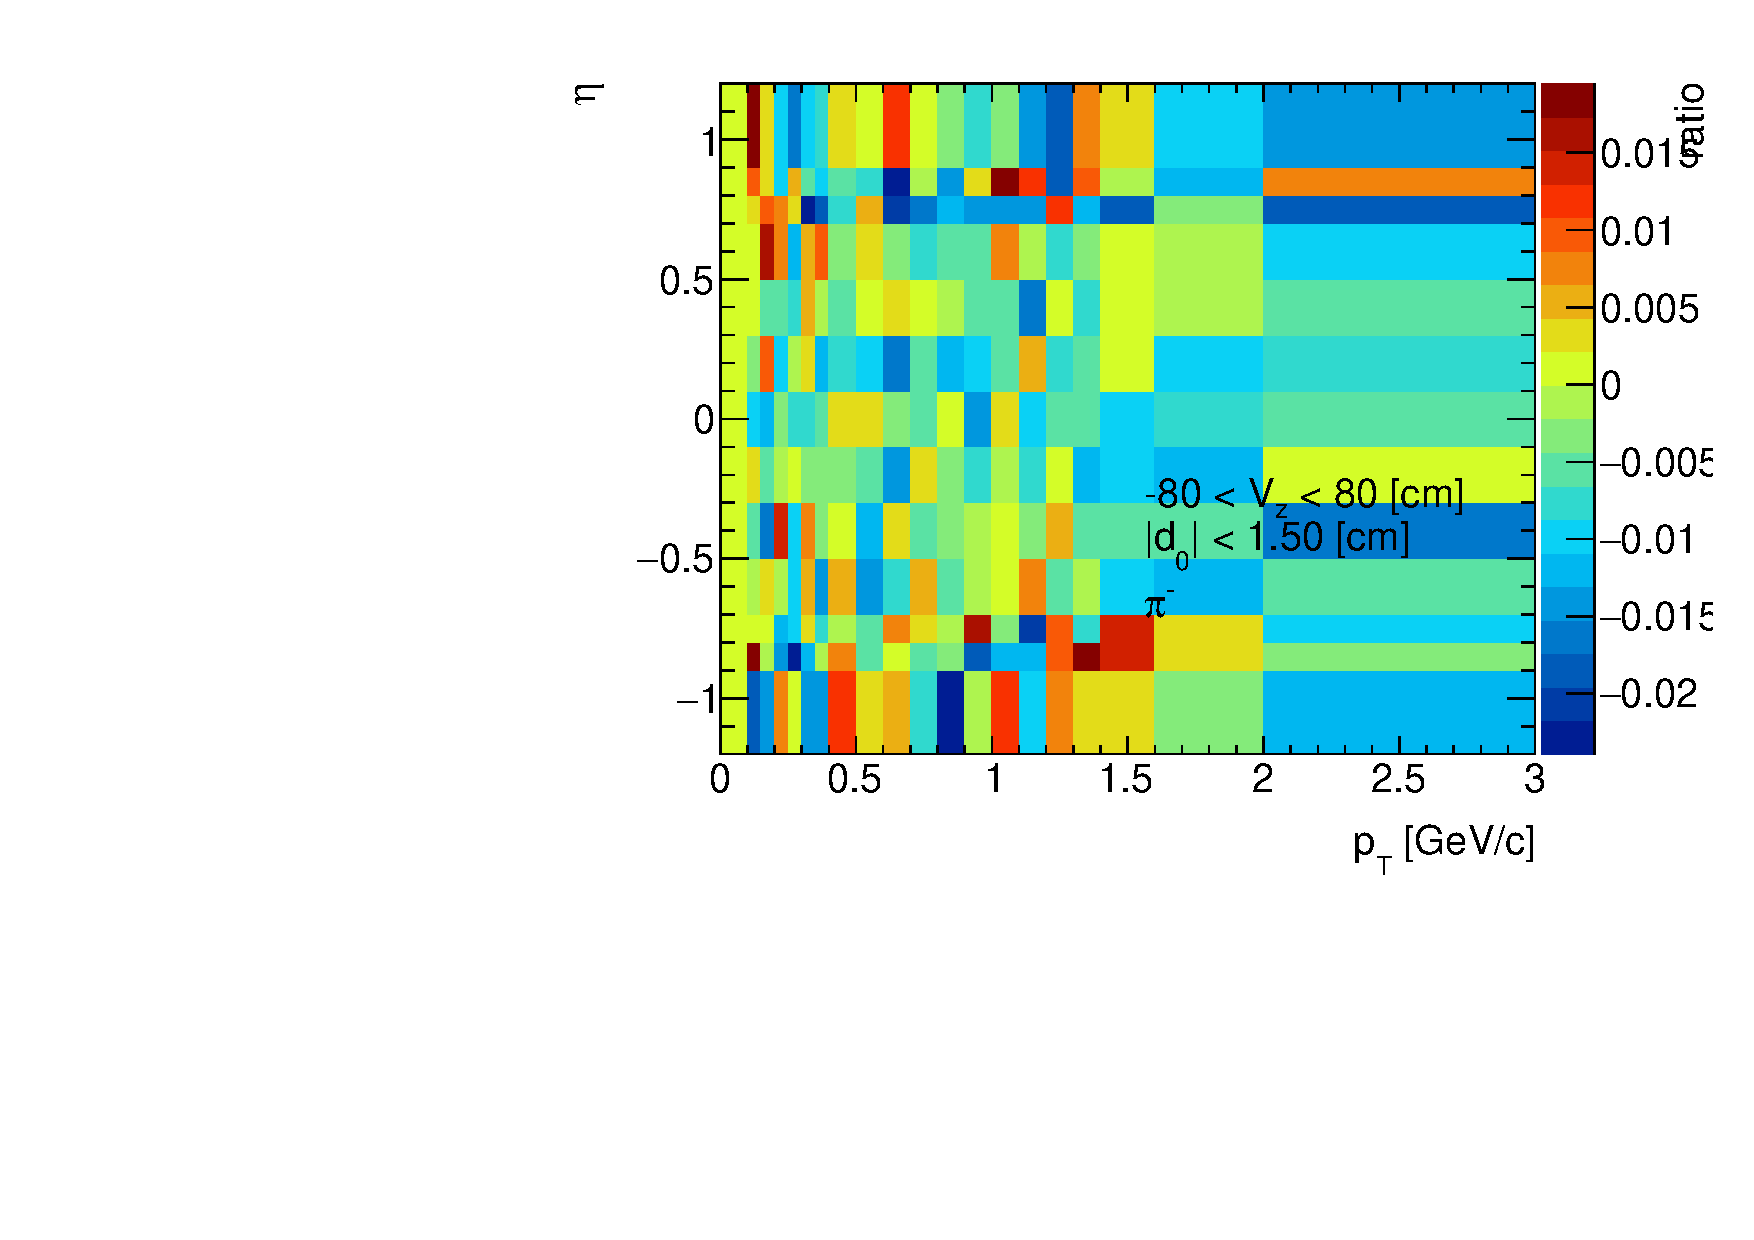
\includegraphics[width=\linewidth,page=1]{graphics/systematicsEfficiency/bbc_and/tofEffi_d0_1_5_etapt_12D.pdf}\\
	}~
	\parbox{0.495\textwidth}{
		\centering
		\includegraphics[width=\linewidth,page=2]{graphics/systematicsEfficiency/bbc_and/tofEffi_d0_1_5_etapt_12D.pdf}\\
	}%
	\caption[The difference $\Delta\epsilon_{ TOF} =\Delta\epsilon_{ TOF}^{1400\text{ kHz}}-2\cdot\Delta\epsilon_{ TOF}^{700\text{ kHz}}$ for $\pi^\pm$ as a function of $p_T$ and $\eta$ $\left(|V_z|<80\text{ cm}\right)$]{The difference $\Delta\epsilon_{ TOF} =\Delta\epsilon_{ TOF}^{1400\text{ kHz}}-2\cdot\Delta\epsilon_{ TOF}^{700\text{ kHz}}$ for $\pi^\pm$ as a function of $p_T$ and $\eta$ $\left(|V_z|<80\text{ cm}\right)$. }
	\label{fig:systError2Dtof}
\end{figure}



\subsection{TOF system simulation accuracy}\label{subsec:tofAbsEffSystAndCorr}

Systematic uncertainty of the TOF efficiency related to the accuracy of the TOF system simulation in STARsim and the data driven correction to it derived in Sec.~\ref{sec:tofAbsEffCorr} was estimated by comparing that nominal TOF efficiency with the one obtained with an independent method described below.

In some STAR analyses the TOF hit reconstruction and matching efficiency is determined from the data with the use of BEMC: real (in-time) tracks are selected based on the fact that they match to BEMC cluster. If they do, the TOF efficiency is calculated as a ratio of number of TOF-matched tracks to number of all tracks. This solution may provide slightly biased efficiency, because the signal in the detector placed behind TOF, such as BEMC, ensures that particle still followed the original helical path past the last hit of the track in TPC (Fig.~\ref{fig:hftEffSketch}). Also, BEMC clusters are more efficiently reconstructed as the energy deposits in the calorimeter increase, which may favor tracks which generated secondaries in front of the BEMC, hence possibly also in front of TOF thus increasing a chance to reconstruct hit in TOF.

To estimate systematic error of the TOF efficiency we decided to calculate efficiency utilizing the TPC tracks containing hits in HFT. The HFT is a group of silicon detectors (PXL, IST, SST) which differ from the gaseous detectors (like TPC) in many aspects. The difference that is most important for this study is the time of response/memory - much shorter in HFT than in TPC. Therefore if the TPC track contain hits in the silicon of HFT it is very probably a real track of particle produced in the proton-proton interaction in the corresponding bunch crossing. With this HFT-tagged tracks we ommit potential bias related to matching with BEMC cluster.

We used the data from st\_ssdmb stream (VPDMB-5-ssd trigger) from the same runs as the data used in our physics analyses. The HFT-tagged tracks were selected as the primary tracks passing the quality cuts \ref{sec:TpcQualityCuts} (only the TPC hits were counted). These tracks were required to contain hits in two HFT layers: IST ans SST, which vastly reduced probability to select an off-time track in TPC (PXL was not used in reconstruction due to problems in firmware). As shown in Fig.~\ref{fig:zVtxHFT}, the $z_{\text{vtx}}$ coverage of the HFT-tagged tracks is limited to about $\pm20$~cm. We imposes cut on the $z$ position of the vertex $|z_{\text{\text{vtx}}}|<20$~cm to remove tracks from the tails, which generally have large $|\eta|$.

Identification of particles was done using the specific energy loss measured in the TPC ($n^{\sigma}$ variables were used). The following requirements were imposed on $n^{\sigma}$ variables in order to select three species of particles whose tracks were selected for the TOF efficiency analysis:
\begin{itemize}
 \item pions:~~~~~$|n^{\sigma}_{\text{pion}}| < 2$,
 \item kaons:~~~~~$-2 < n^{\sigma}_{\text{proton}} < 2.5$~~~\&\&~~~$|n^{\sigma}_{\text{pion}}| > 3.5$~~~\&\&~~~$|n^{\sigma}_{\text{electron}}| > 3.5$~~~\&\&~~~$|n^{\sigma}_{\text{proton}}| > 3.5$,
 \item protons:~~$-2 < n^{\sigma}_{\text{proton}} < 3$~~~~~\&\&~~~~$|n^{\sigma}_{\text{pion}}| > 3.5$~~~\&\&~~~$|n^{\sigma}_{\text{electron}}| > 3.5$~~~\&\&~~~$|n^{\sigma}_{\text{kaon}}| > 3.5$.
\end{itemize}

%---------------------------
\begin{figure}[b!]%\vspace{-2pt}%
\centering%
\begin{minipage}{.4725\textwidth}%
  \centering%\vspace{11pt}
  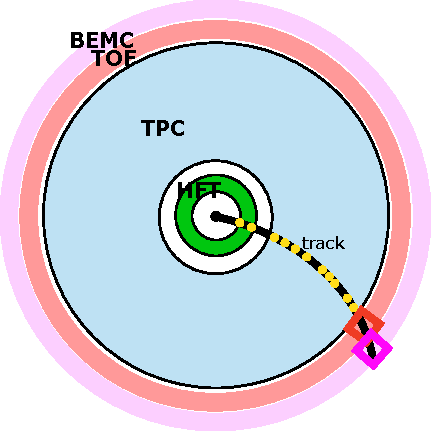
\includegraphics[width=0.965\linewidth]{graphics/systematicsEfficiency/TofSyst/effSketch.pdf}%\vspace{-5pt}%
  \caption[Sketch of the track with points in HFT.]%
  {Sketch of the cross section of the central detector and the track reconstructed with points in HFT. Presence of HFT points in a reconstructed track can be used as a tagger of the in-time tracks.}
  \label{fig:hftEffSketch}
\end{minipage}%
\quad\quad%
\begin{minipage}{.4725\textwidth}%
  \centering%
  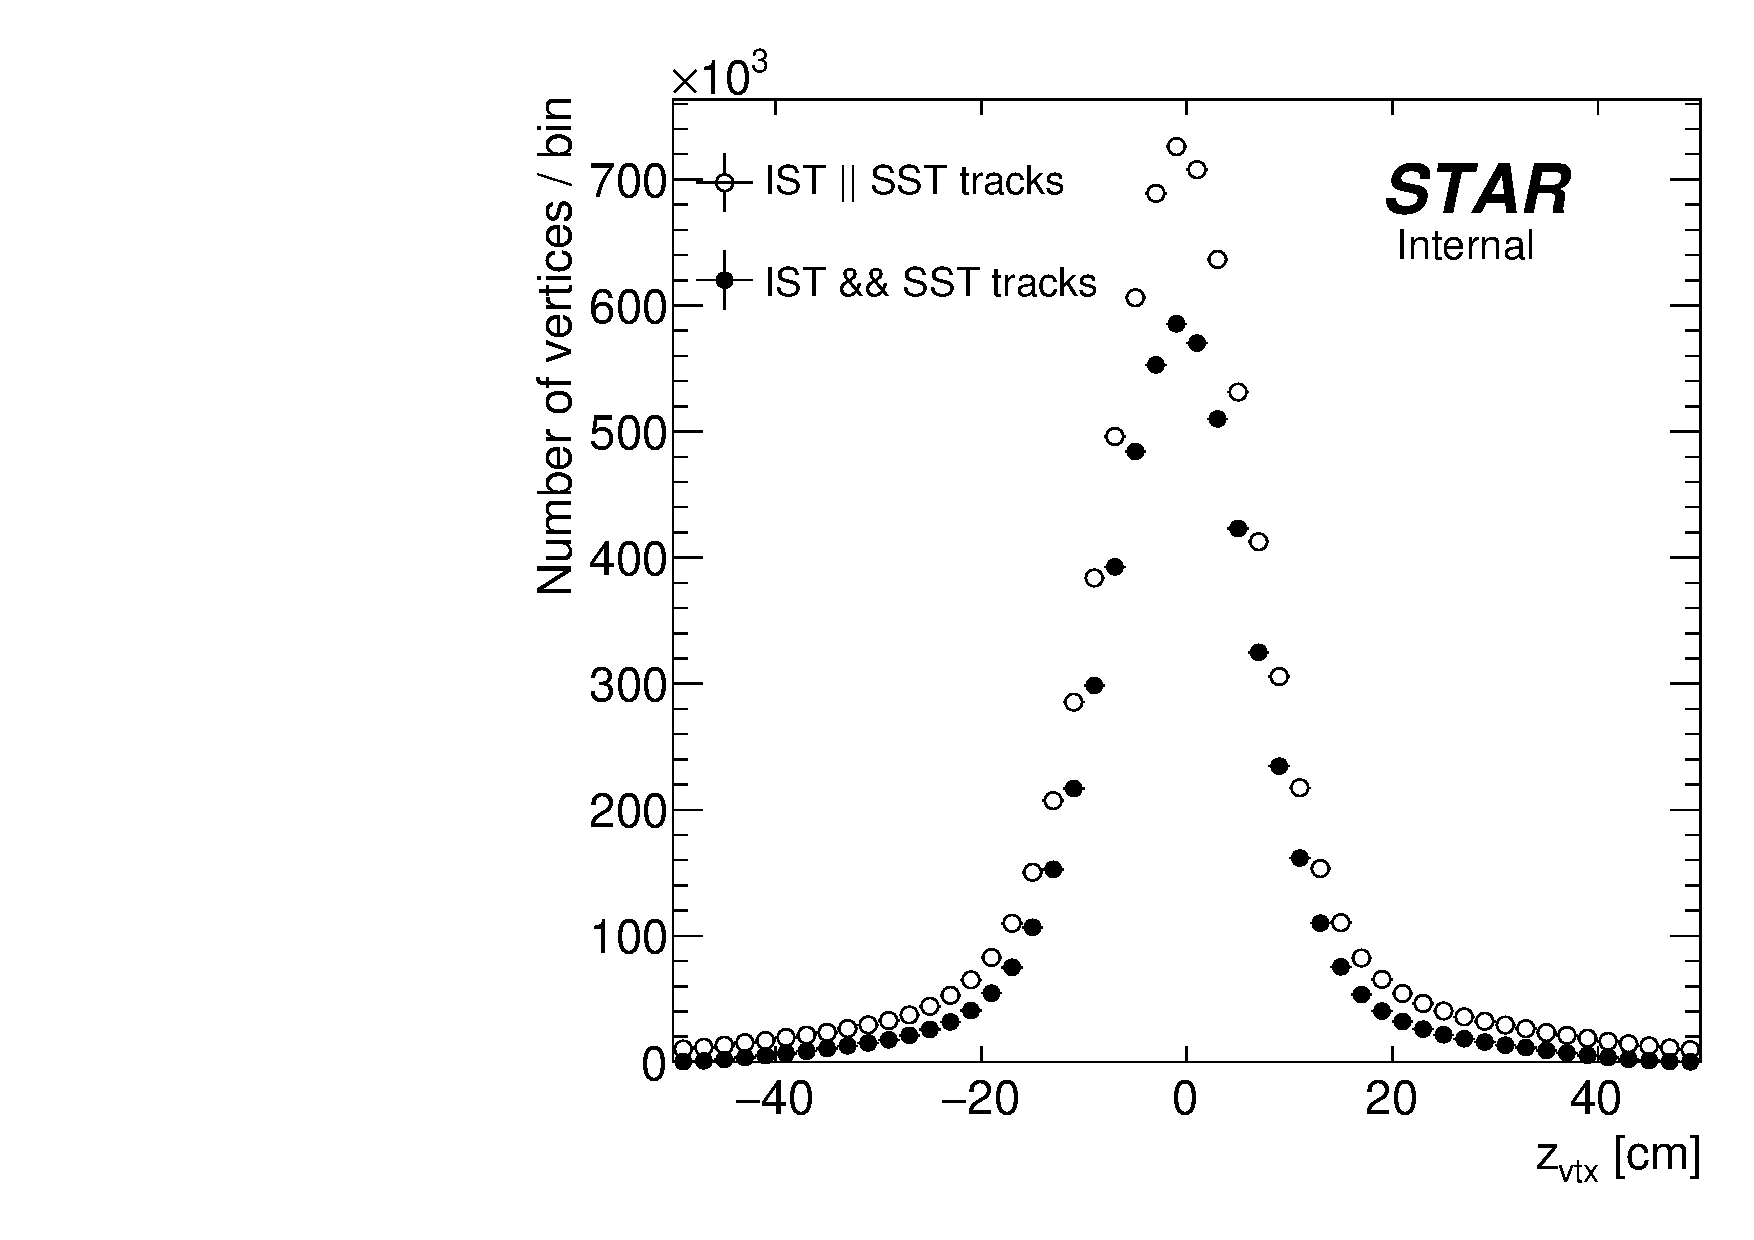
\includegraphics[width=\linewidth]{graphics/systematicsEfficiency/TofSyst/zVtxHFT.pdf}%\vspace*{-5pt}
  \caption[Distribution of $z$-position of vertices with TPC tracks containing hits in HFT.]
   {Distribution of $z$-position of vertices containing TPC tracks with HFT hits (st\_ssd stream). Open circles represent vertices with tracks with hits in IST or SST, full circles - IST and SST.}
   \label{fig:zVtxHFT}%\vspace*{-29pt} 
\end{minipage}%
\end{figure}%
%---------------------------  

\noindent Selection of pions by cut solely on $n^{\sigma}_{\text{pion}}$ (without additional cuts on $n^{\sigma}$ for kaon, proton and electron hypothesis) is driven by the dominance of pion production over other species and by the fact that the dE/dx of pions overlap with kaons and protons at momenta which are relatively large, hence the TOF efficiency is saturated and the same for all particle species. More sophisticated selection was used for kaons and protons. Figure~\ref{fig:hftTracksNSigmaVsPt} shows the $n^{\sigma}$ variables before and after the selection of kaons (\ref{fig:hftTracksNSigmaKaonVsPt}) and protons (\ref{fig:hftTracksNSigmaProtonVsPt}), where one can find proof that clean samples of these particles were selected, for the price of limited coverage in track $p_{T}$.
%---------------------------
\begin{figure}[t!]
\centering
\parbox{0.4725\textwidth}{
  \centering
  \begin{subfigure}[b]{\linewidth}
                \subcaptionbox{\label{fig:hftTracksNSigmaKaonVsPt}}{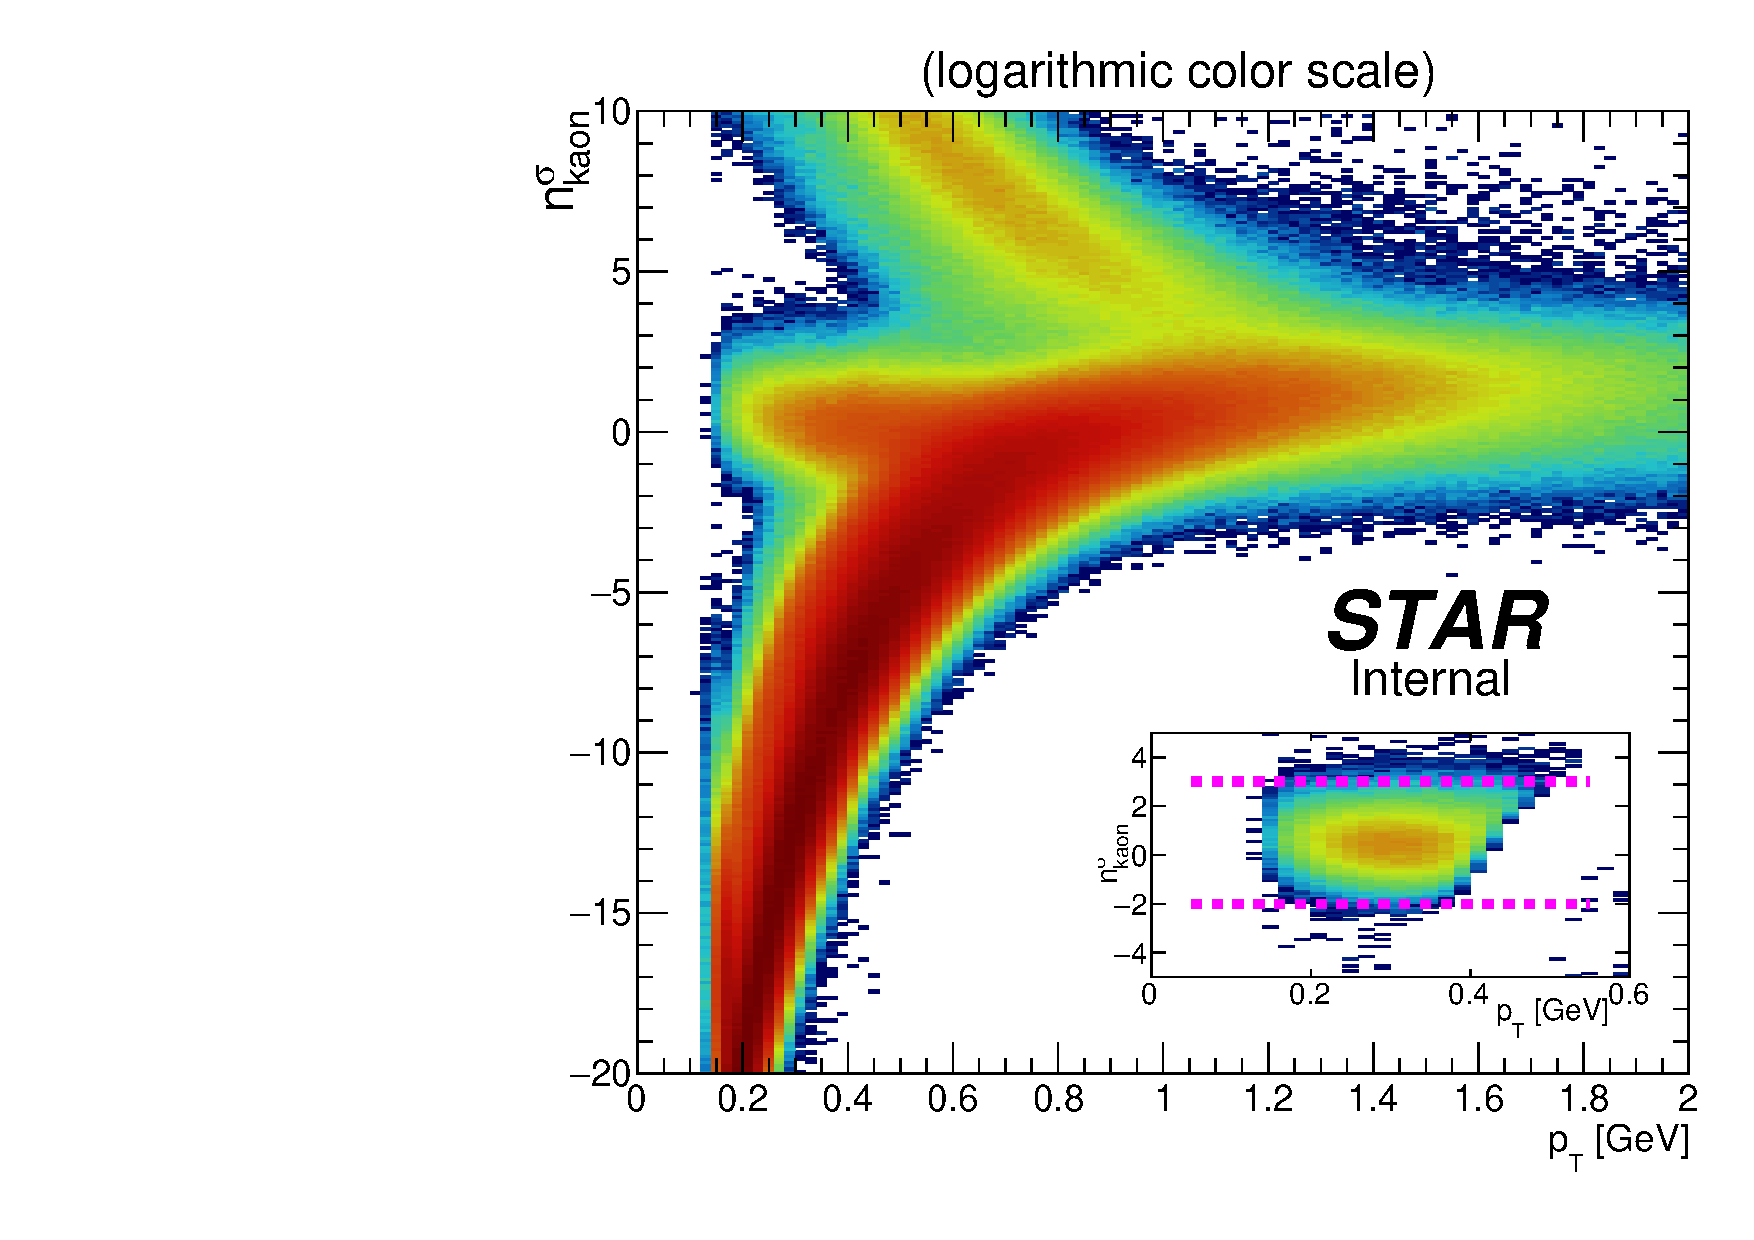
\includegraphics[width=\linewidth]{graphics/systematicsEfficiency/TofSyst/NSigmaKaonVsPt.pdf}}\vspace{-5pt}
  \end{subfigure}
}%
\quad\quad%
\parbox{0.4725\textwidth}{
  \centering
  \begin{subfigure}[b]{\linewidth}
                \subcaptionbox{\label{fig:hftTracksNSigmaProtonVsPt}}{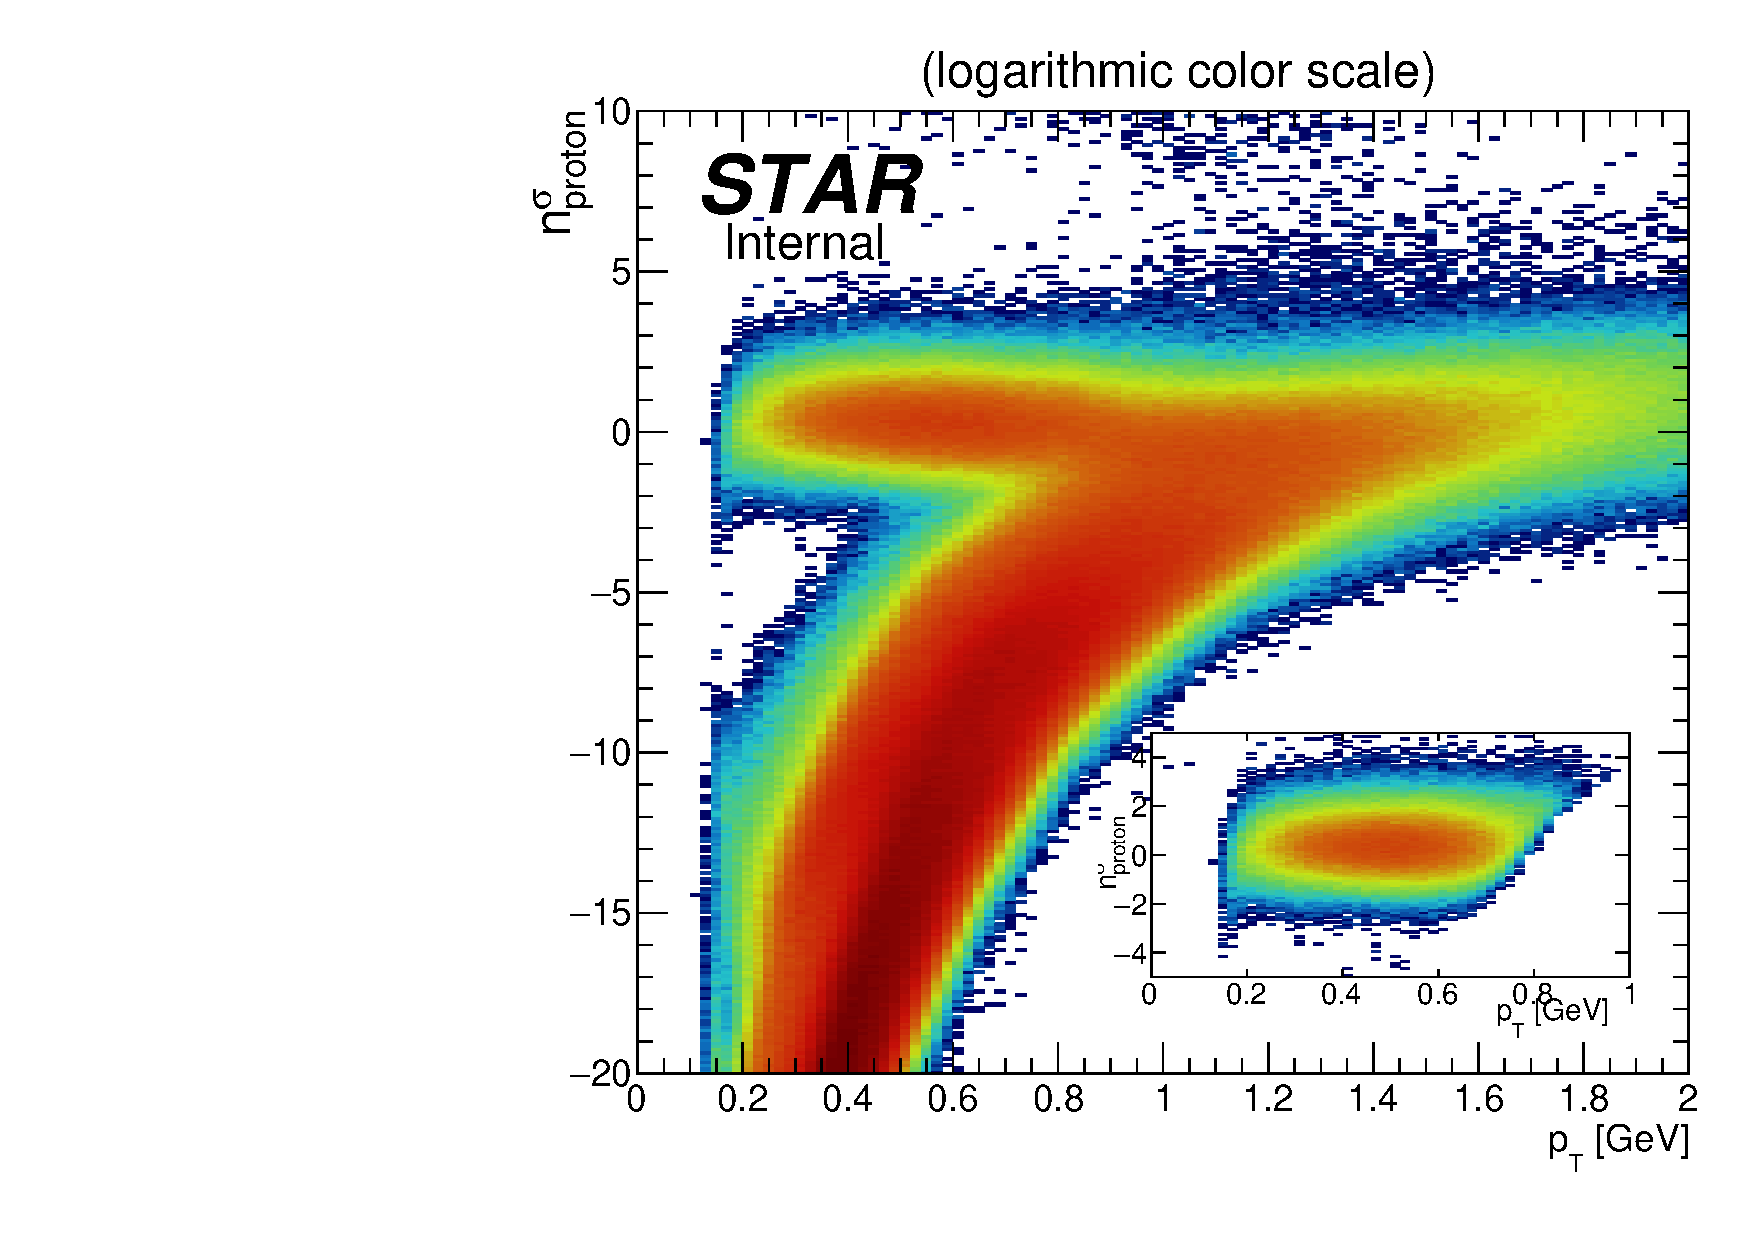
\includegraphics[width=\linewidth]{graphics/systematicsEfficiency/TofSyst/NSigmaProtonVsPt.pdf}}\vspace{-5pt}
  \end{subfigure}
}%
\caption[Distribution of $n^{\sigma}$ (kaon and proton) vs. transverse momentum for tracks containing HFT hits.]%
    {Distribution of $n^{\sigma}_{\text{kaon}}$ (\ref{fig:hftTracksNSigmaKaonVsPt}) and $n^{\sigma}_{\text{proton}}$ (\ref{fig:hftTracksNSigmaProtonVsPt}) vs. track $p_{T}$ for tracks containing HFT hits. The insert in each subfigure shows the corresponding $n^{\sigma}$ vs. $p_{T}$ distribution after preselection of tracks of given spiecies (without cut on variable in $y$-axis) according to description provided in the text in preceding page. Dashed magenta lines represent final cuts on corresponding $n^{\sigma}$ quantity used to select tracks of given species.}\label{fig:hftTracksNSigmaVsPt}%
\end{figure}
%---------------------------

%---------------------------
\begin{figure}[b!]\vspace{-34pt}
\centering
\parbox{0.31\textwidth}{
  \centering
  \begin{subfigure}[b]{\linewidth}{
                \subcaptionbox{\label{fig:TPcorrectionTofEff2D}}{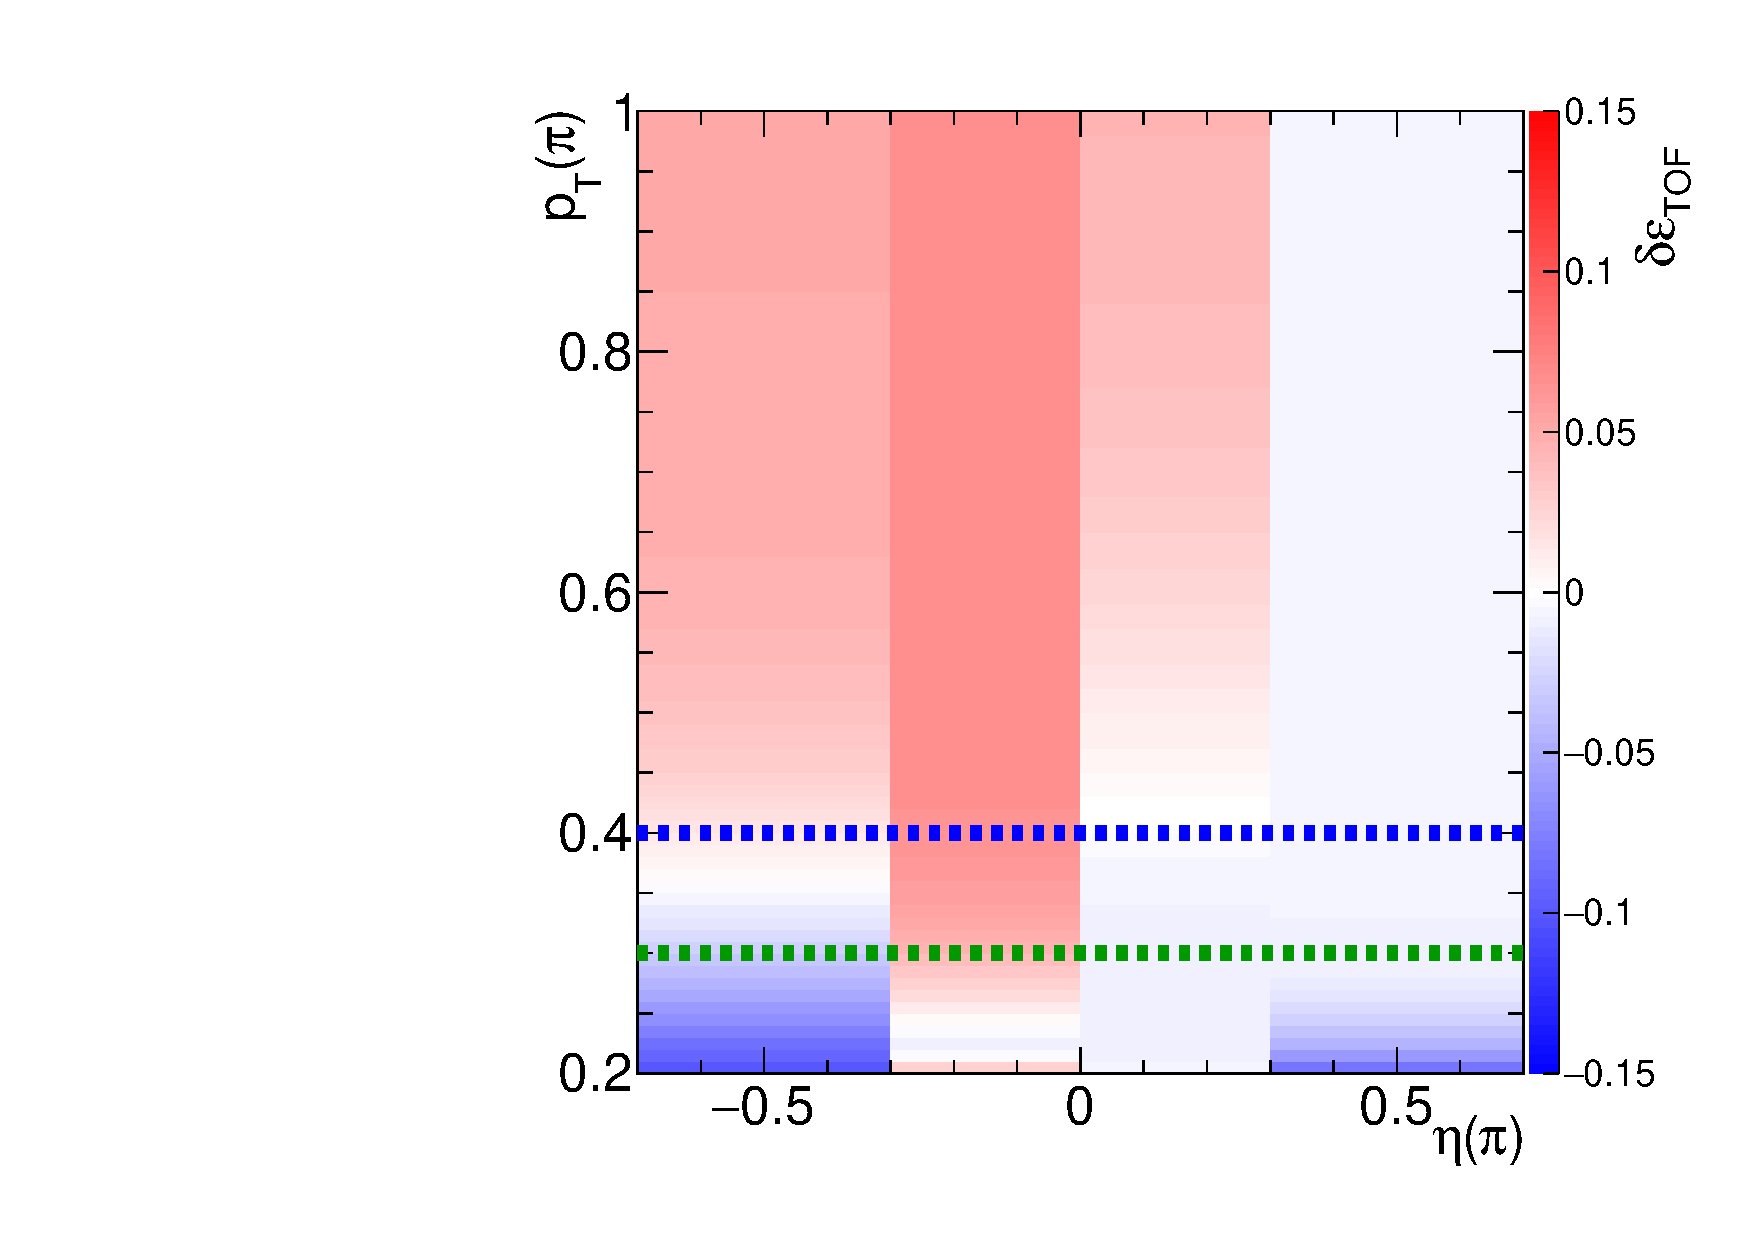
\includegraphics[width=\linewidth]{graphics/systematicsEfficiency/TofSyst/TofEffCorrection2D_pion.pdf}\vspace{-12pt}}}
  \end{subfigure} 
} 
\quad
\parbox{0.65\textwidth}{ 
  \centering
		\begin{minipage}[t][0.64\linewidth][t]{\linewidth}\vspace{73pt}
			\caption[Comparison of the TOF eff. correction from tag\&probe method and the difference between TOF eff. calculated using standard method from the HFT-tagged tracks and efficiency from embedded single particle MC.]%
    {Comparison of the TOF efficiency correction obtained with tag\&probe method on CEP $\pi^{+}\pi^{-}$ events (\ref{fig:TPcorrectionTofEff2D}, description in Sec.~\ref{sec:tofAbsEffCorr}) and the difference between TOF efficiency calculated using standard method from the HFT-tagged tracks and efficiency from embedded single particle MC for pions (\ref{fig:tofEffDifference_pion}), kaons (\ref{fig:tofEffDifference_kaon}) and protons (\ref{fig:tofEffDifference_proton}). Yellow hatched area mark empty bins. Dashed horizontal lines represent minimum track $p_{T}$ thresholds used in our analyses: $0.3$~GeV for kaons (green) and $0.4$~GeV for protons (blue).}\label{fig:tofEffSystematics2DComparison}% 
		\end{minipage}
}\\[-25pt]
\parbox{0.31\textwidth}{
  \centering
  \begin{subfigure}[b]{\linewidth}{
                \subcaptionbox{\label{fig:tofEffDifference_pion}}{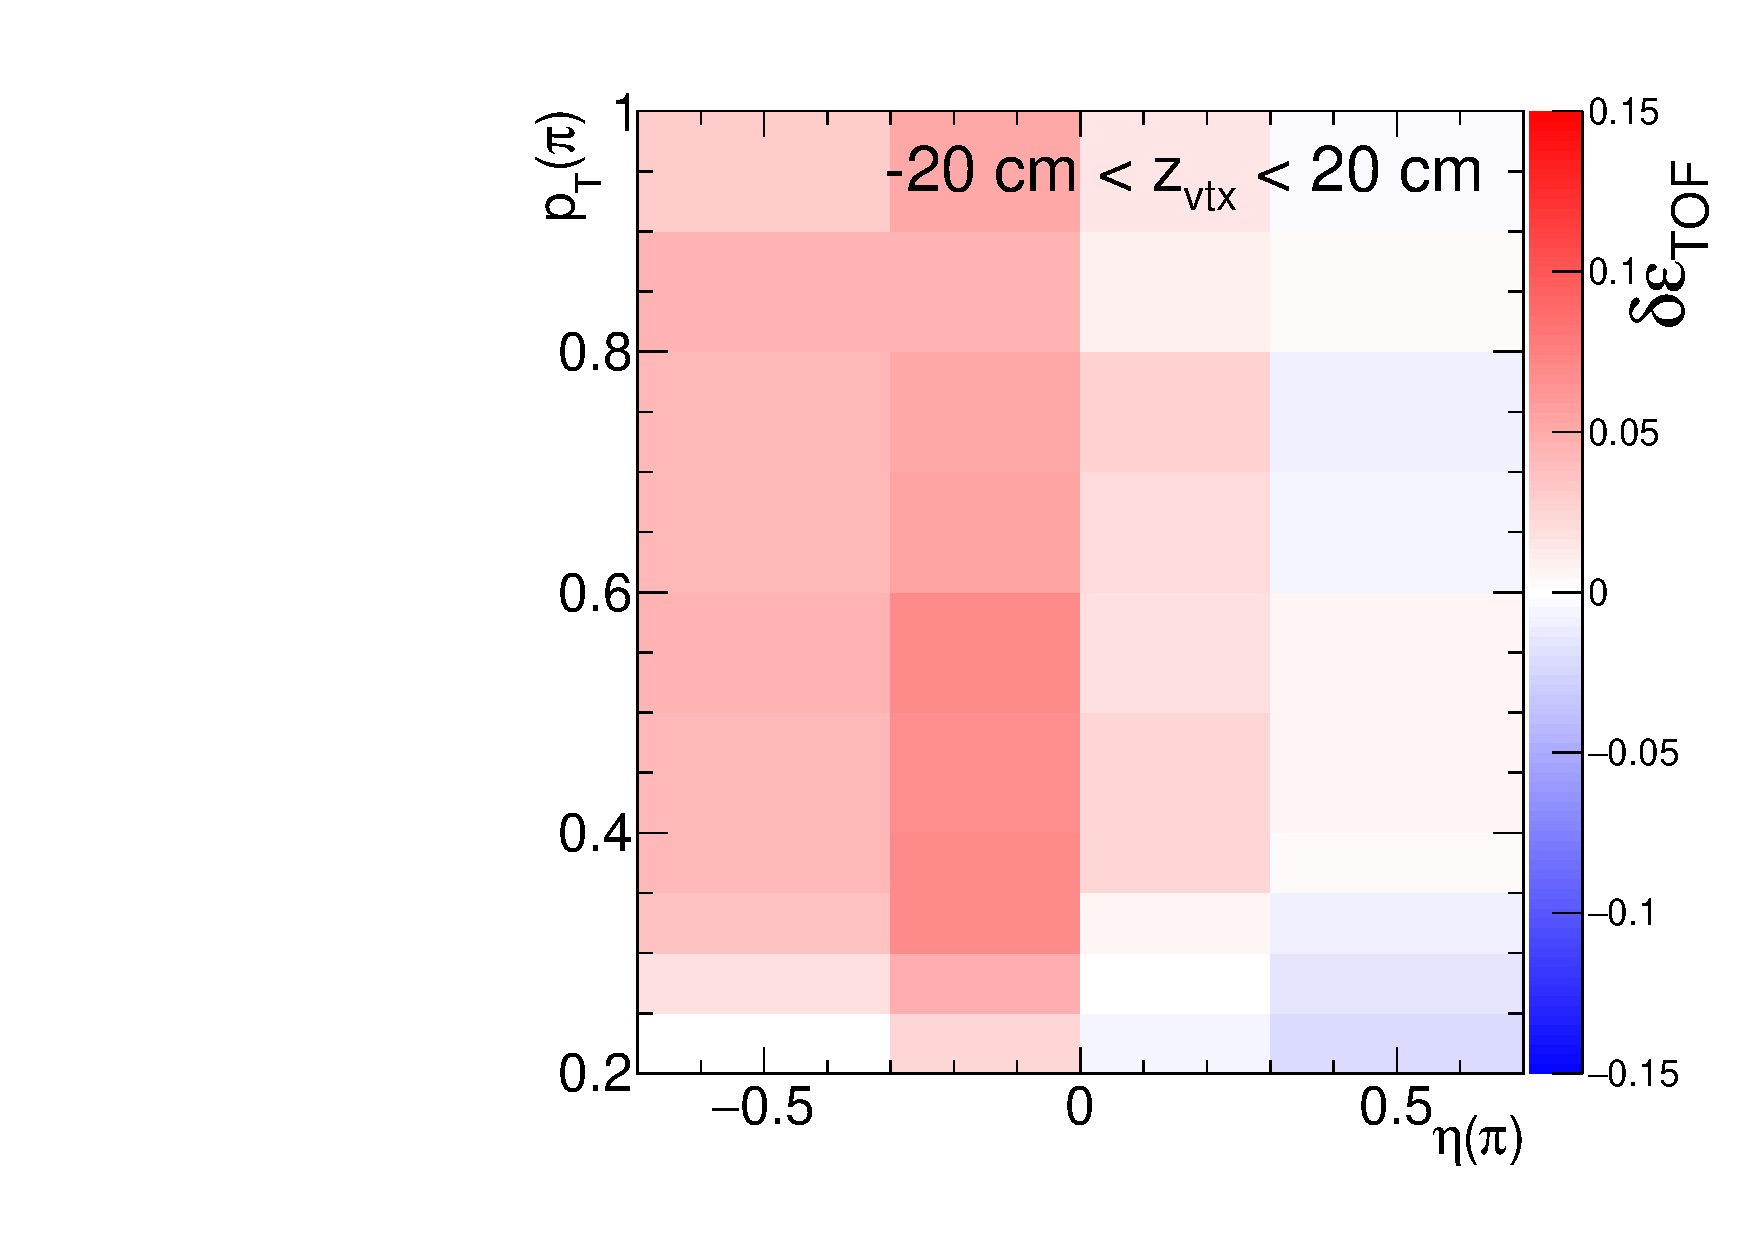
\includegraphics[width=\linewidth]{graphics/systematicsEfficiency/TofSyst/tofEffDifference_pion.pdf}\vspace{-12pt}}}
  \end{subfigure}
}
\quad
\parbox{0.31\textwidth}{
  \centering
  \begin{subfigure}[b]{\linewidth}{
                \subcaptionbox{\label{fig:tofEffDifference_kaon}}{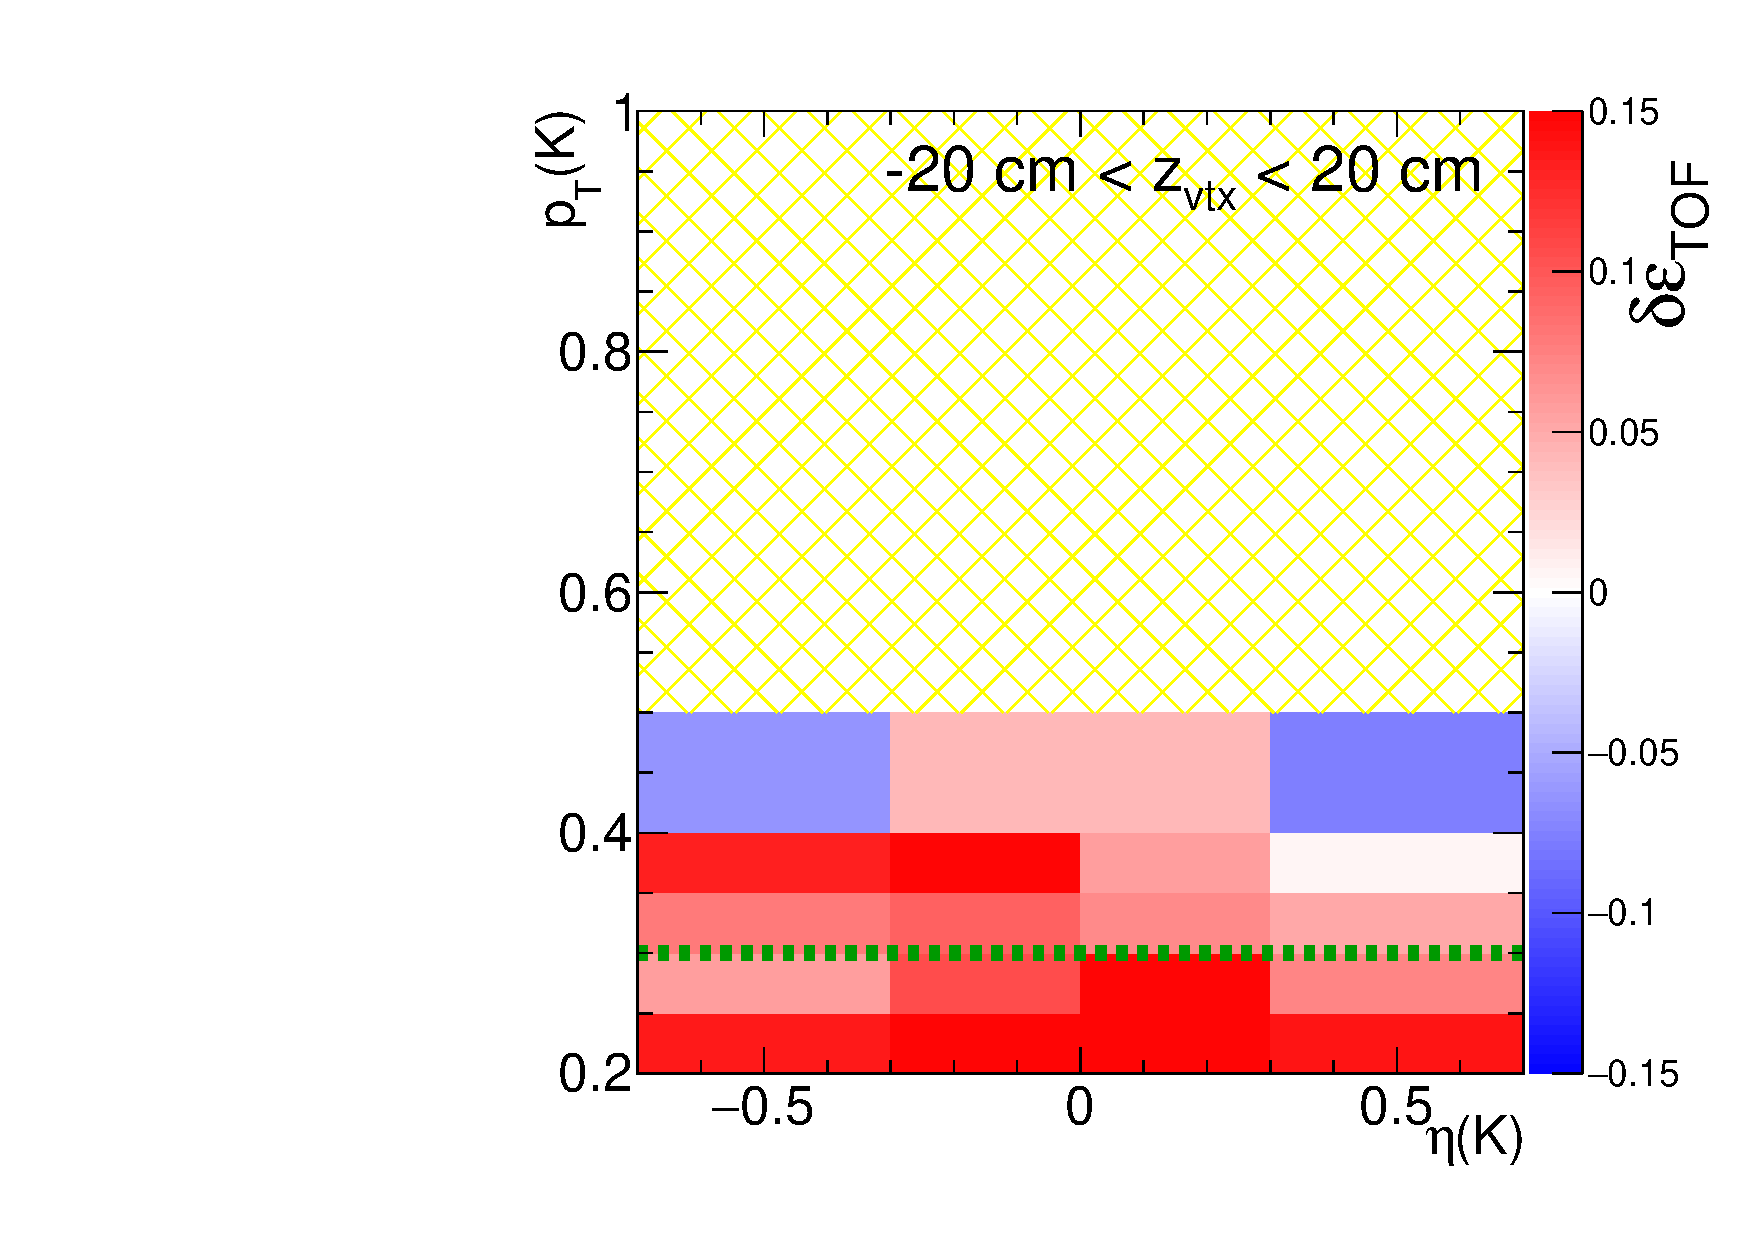
\includegraphics[width=\linewidth]{graphics/systematicsEfficiency/TofSyst/tofEffDifference_kaon.pdf}\vspace{-12pt}}}
  \end{subfigure}
} 
\quad
\parbox{0.31\textwidth}{
  \centering
  \begin{subfigure}[b]{\linewidth}{
                \subcaptionbox{\label{fig:tofEffDifference_proton}}{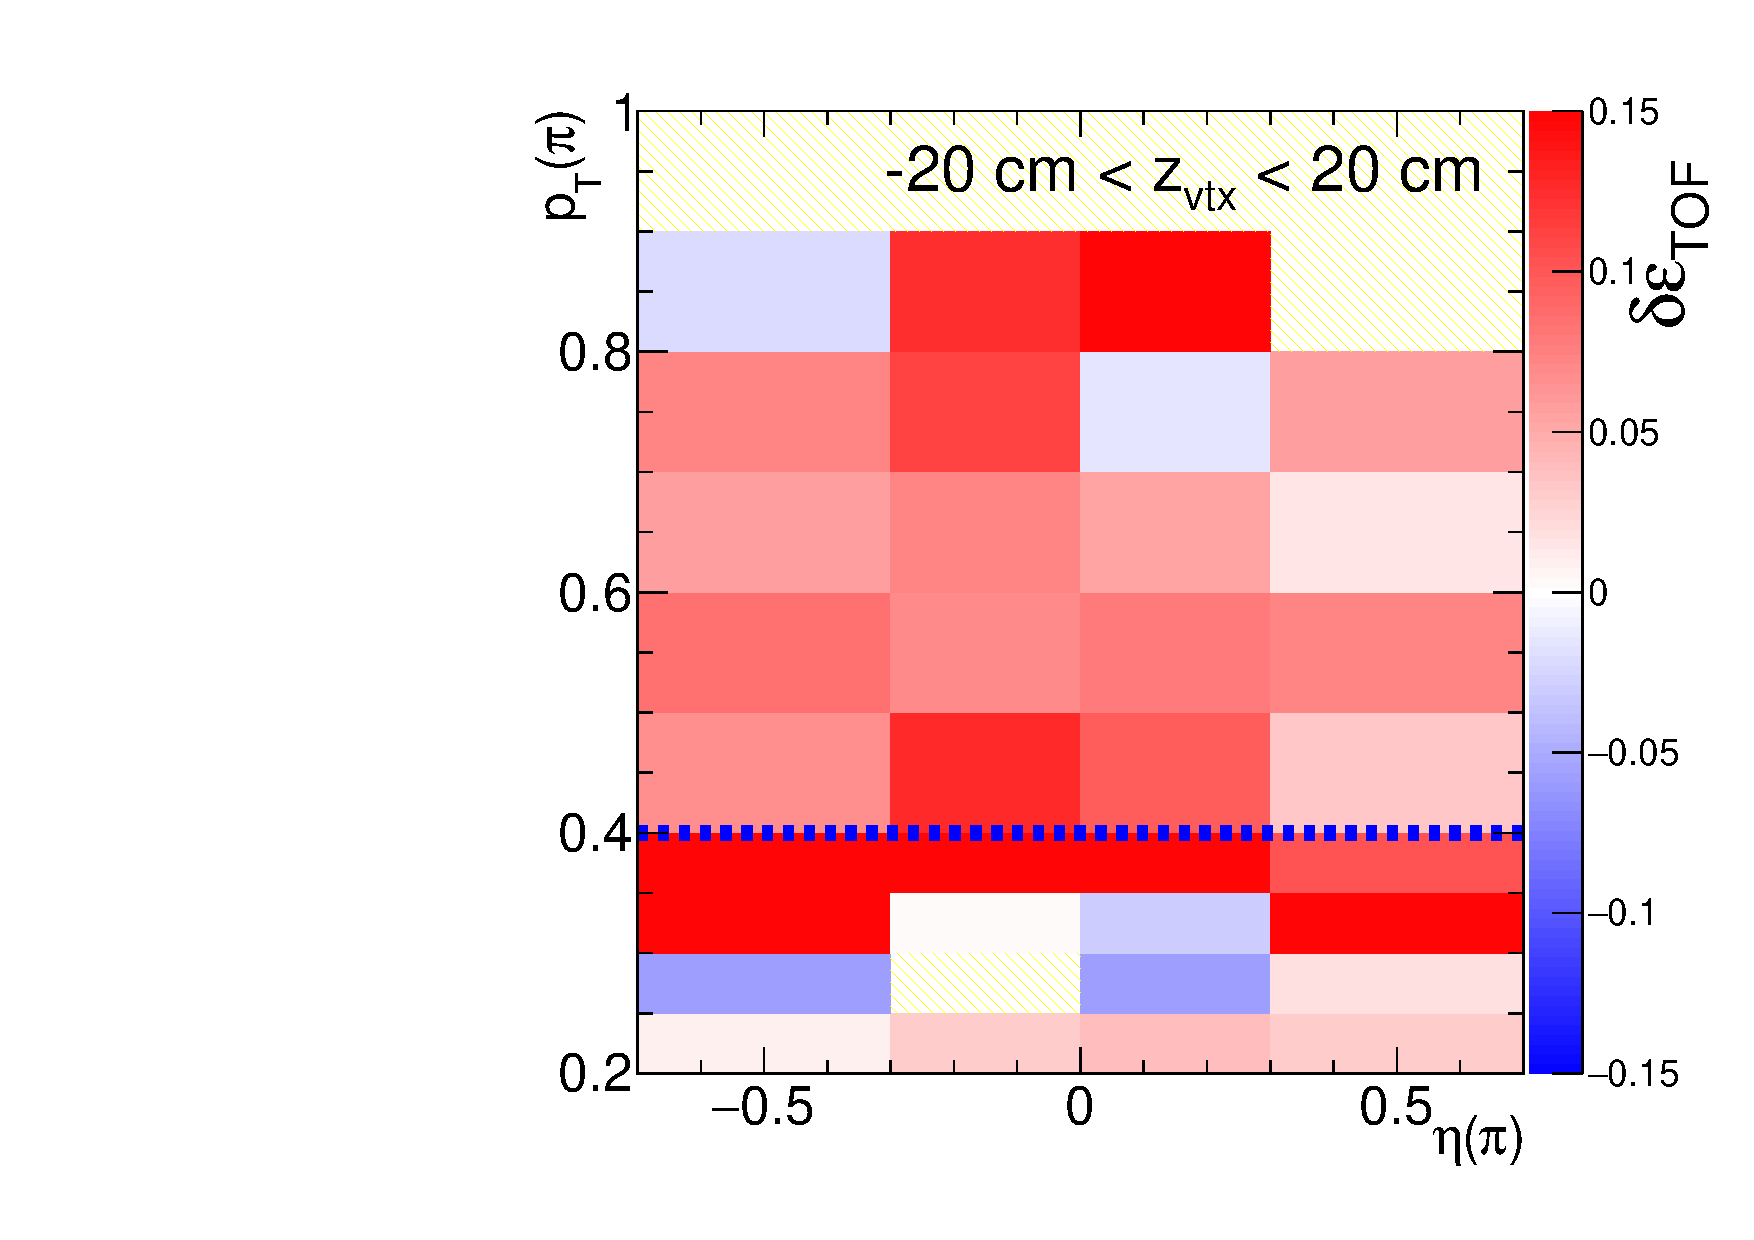
\includegraphics[width=\linewidth]{graphics/systematicsEfficiency/TofSyst/tofEffDifference_proton.pdf}\vspace{-12pt}}}
  \end{subfigure}
}

\end{figure}
%---------------------------


From selected sample of pion, kaon and proton tracks the TOF hit reconstruction and matching efficiency was calculated using the standard method - as a ratio of number of tracks matched with TOF and number of all tracks. This efficiency was compared with the efficiency extracted from the zero-bias-embedded single particle MC, calculated for $|z_{\text{vtx}}|<20$~cm and averaged between positive- and negative-charge particles. The result of comparison - the difference between efficiency calculated with HFT-tagged tracks and efficiency from single particle MC, is presented in Fig.~\ref{fig:tofEffSystematics2DComparison} (subfigures \ref{fig:tofEffDifference_pion}-\ref{fig:tofEffDifference_proton}). This difference could be interpreted as a data-driven correction to the TOF efficiency calculated from single particle MC, alternative to correction derived with tag\&probe method on CEP events, described in Sec.~\ref{sec:tofAbsEffCorr}.

The difference between the correction from tag\&probe (Fig.\ref{fig:TPcorrectionTofEff2D}) and alternative correction in Figs.~\ref{fig:tofEffDifference_pion}-\ref{fig:tofEffDifference_proton}, $\Delta\delta\varepsilon_{\text{TOF}}$, can be used as a measure of the uncertainty of the overall TOF efficiency. Aforementioned difference is depicted in Fig.~\ref{fig:tofEffDifference_Delta}. We decided to symmetrize the systematic uncertainty of the TOF efficiency. For this purpose, on top of the correction to the TOF efficiency from CEP tag\&probe method, we add the half of the difference from Fig.~\ref{fig:tofEffDifference_Delta} to the TOF efficiency of corresponding particle type. We then assign a systematic uncertainty of the TOF efficiency to each $(\eta,p_{T})$ bin as an absolute value of the half of that difference, $\frac{1}{2}|\Delta\delta\varepsilon_{\text{TOF}}|$. We assume that the systematic uncertainty for tracks whose $|z_{\text{vtx}}|>20$~cm is the same as for HFT tracks studied here ($|z_{\text{vtx}}|<20$!~cm). For high track $p_{T}$, when there are no estimates of $\Delta\delta\varepsilon_{\text{TOF}}$, the value from the last non-empty $p_{T}$ bin (at given $\eta$ bin) is used as a correction, and maximum absolute value among the last 3 non-empty $p_{T}$ bins (at given $\eta$ bin) is used as a systematic uncertainty.

%---------------------------
\begin{figure}[h]%\vspace{-38pt} 
\centering
\parbox{0.31\textwidth}{
  \centering
  \begin{subfigure}[b]{\linewidth}{
                \subcaptionbox{\label{fig:tofEffDifference_Delta_pion}}{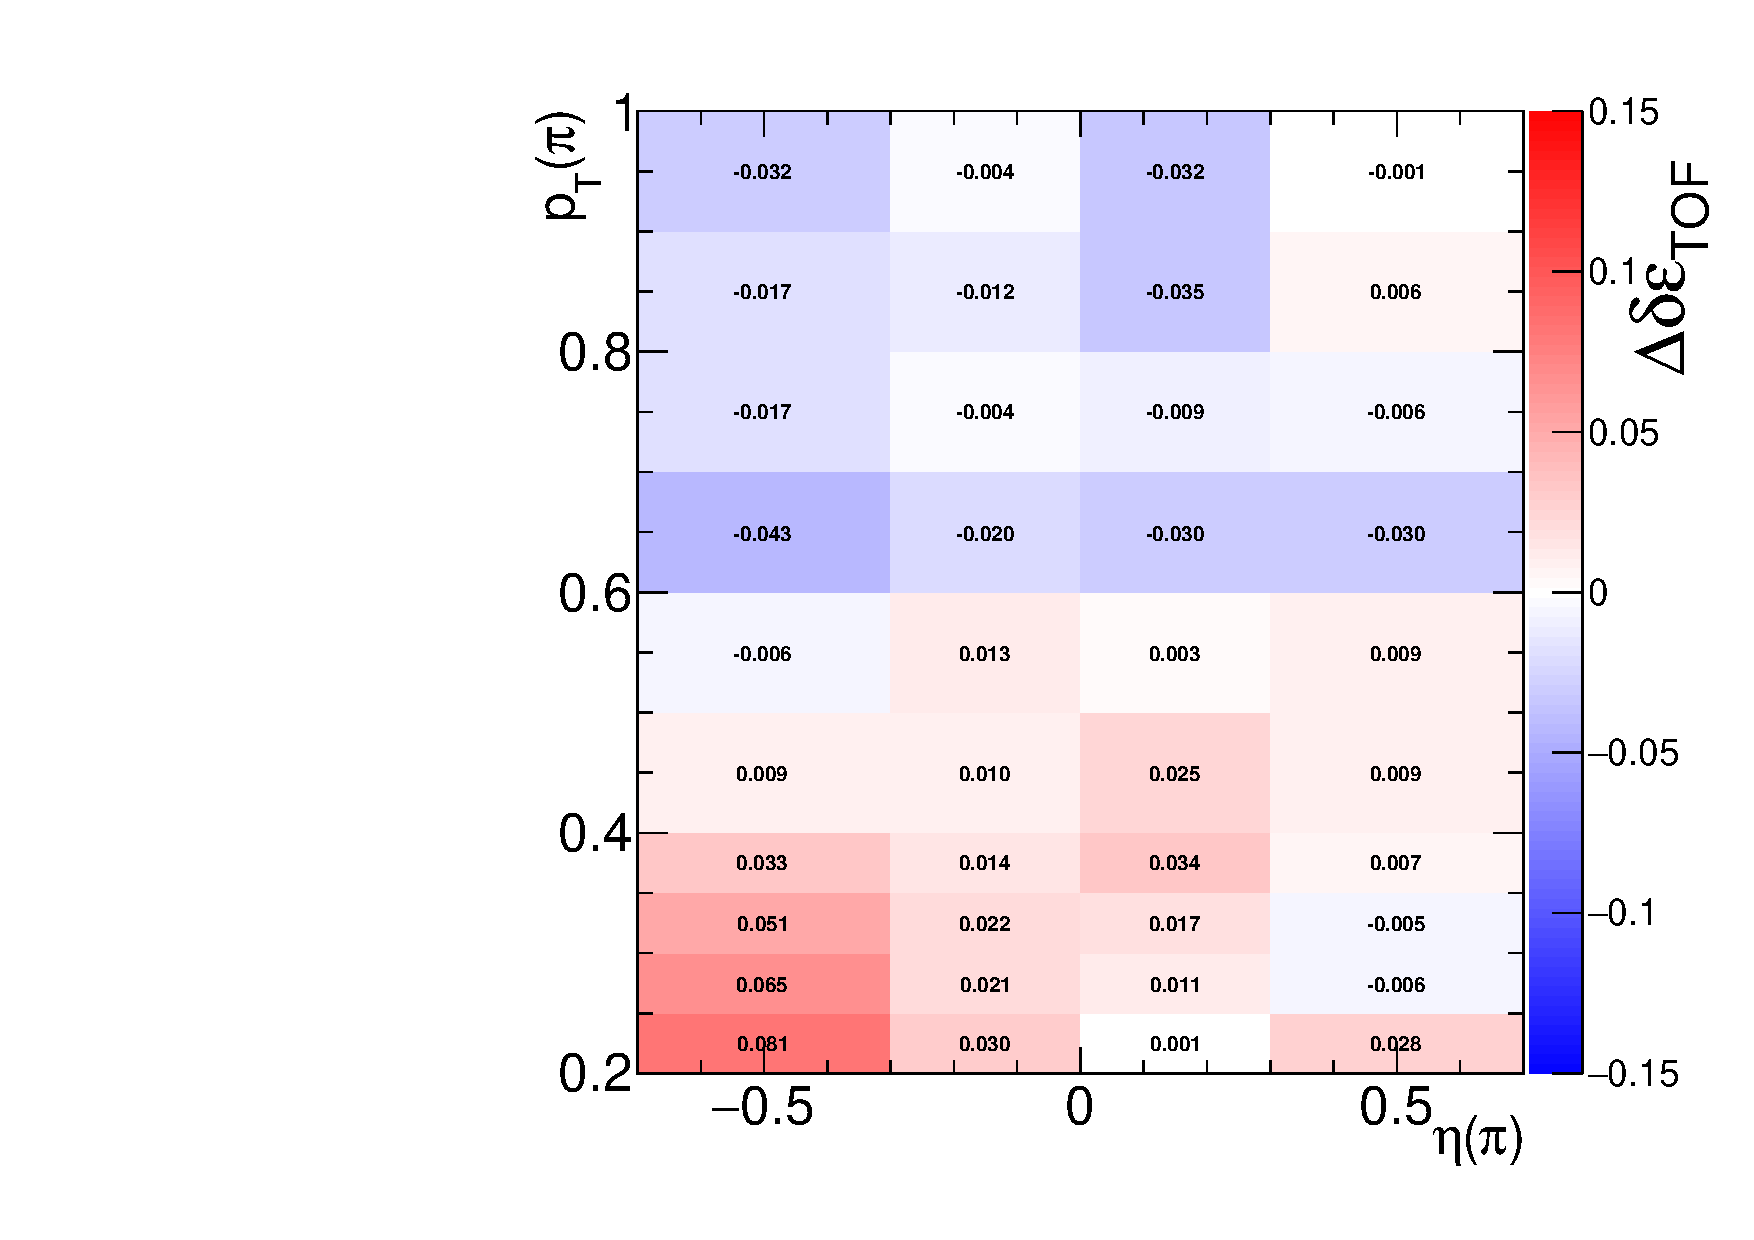
\includegraphics[width=\linewidth]{graphics/systematicsEfficiency/TofSyst/tofEffDifference_Delta_pion.pdf}\vspace{-12pt}}}
  \end{subfigure}
}
\quad
\parbox{0.31\textwidth}{
  \centering
  \begin{subfigure}[b]{\linewidth}{
                \subcaptionbox{\label{fig:tofEffDifference_Delta_kaon}}{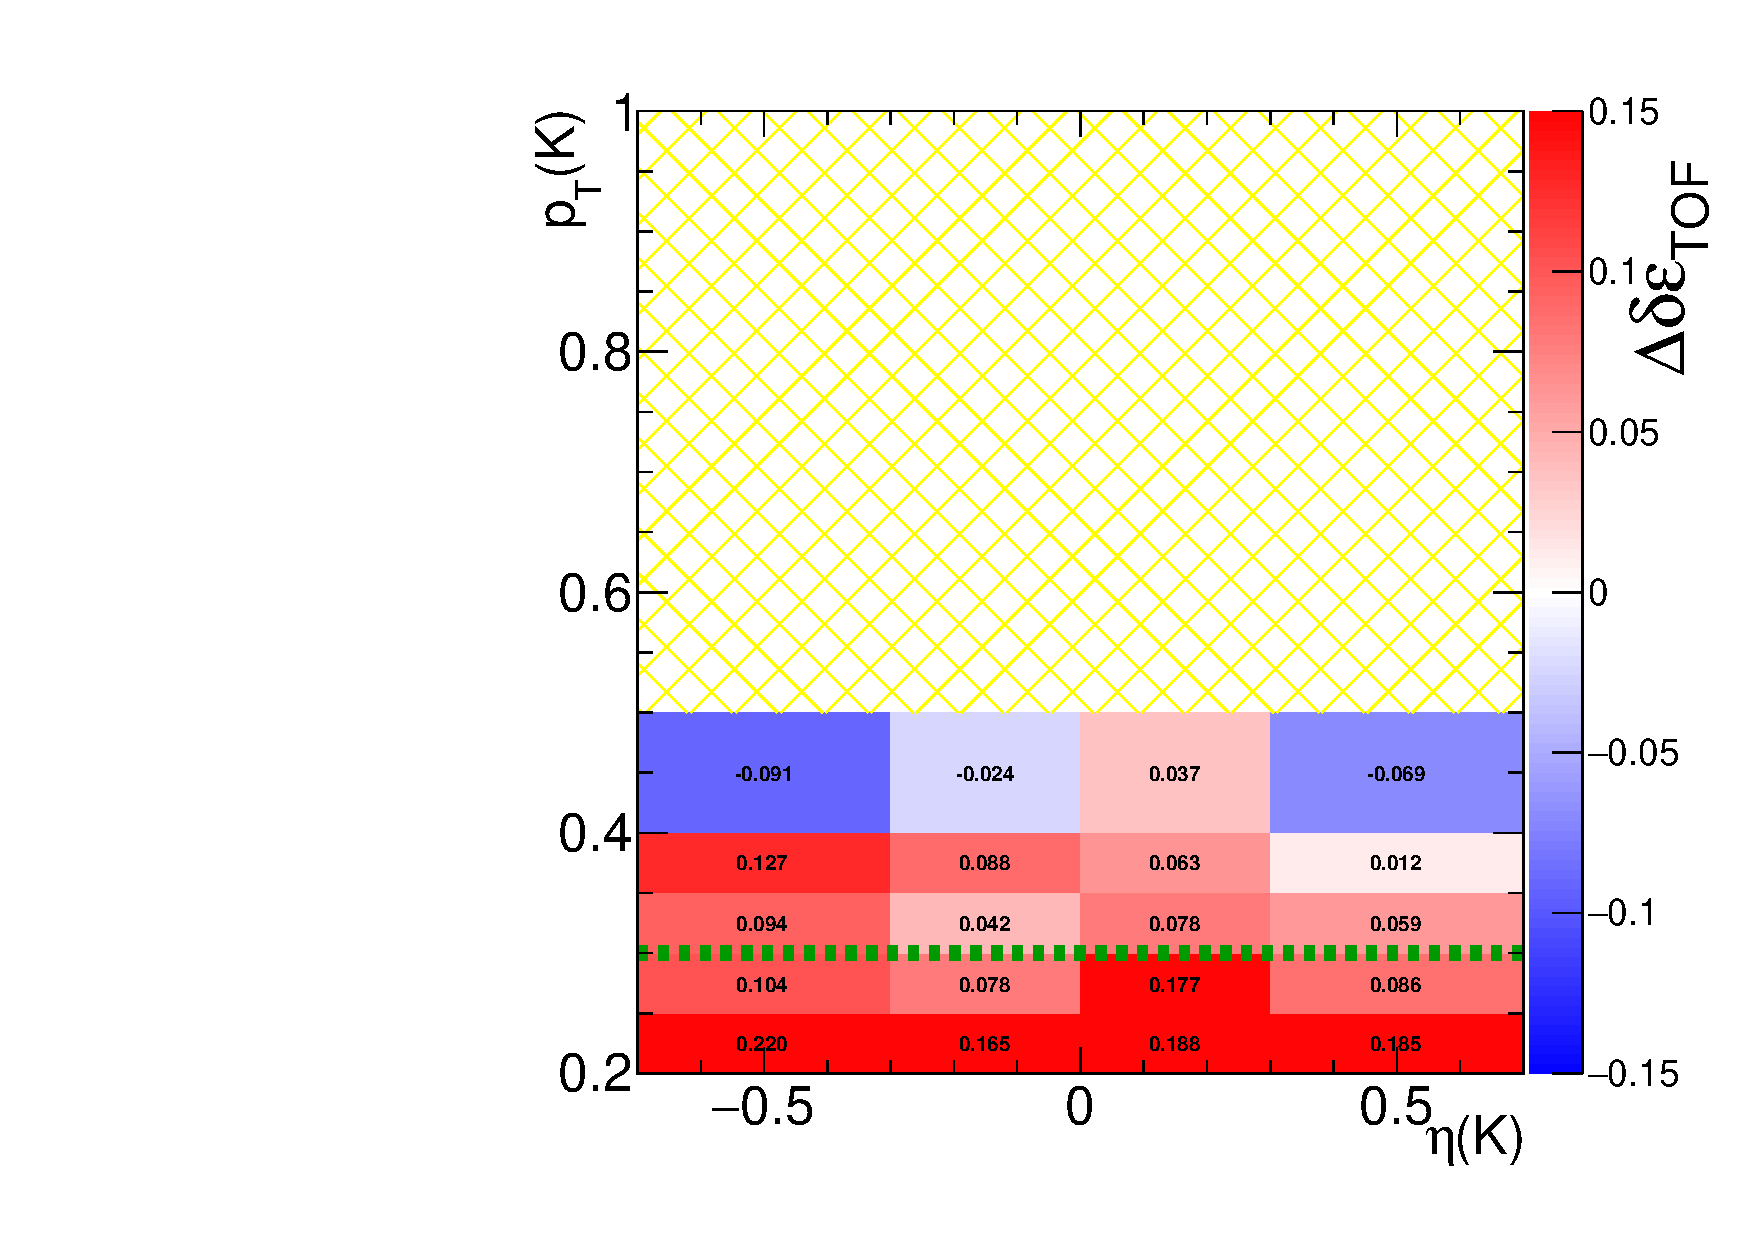
\includegraphics[width=\linewidth]{graphics/systematicsEfficiency/TofSyst/tofEffDifference_Delta_kaon.pdf}\vspace{-12pt}}}
  \end{subfigure}
} 
\quad
\parbox{0.31\textwidth}{
  \centering
  \begin{subfigure}[b]{\linewidth}{
                \subcaptionbox{\label{fig:tofEffDifference_Delta_proton}}{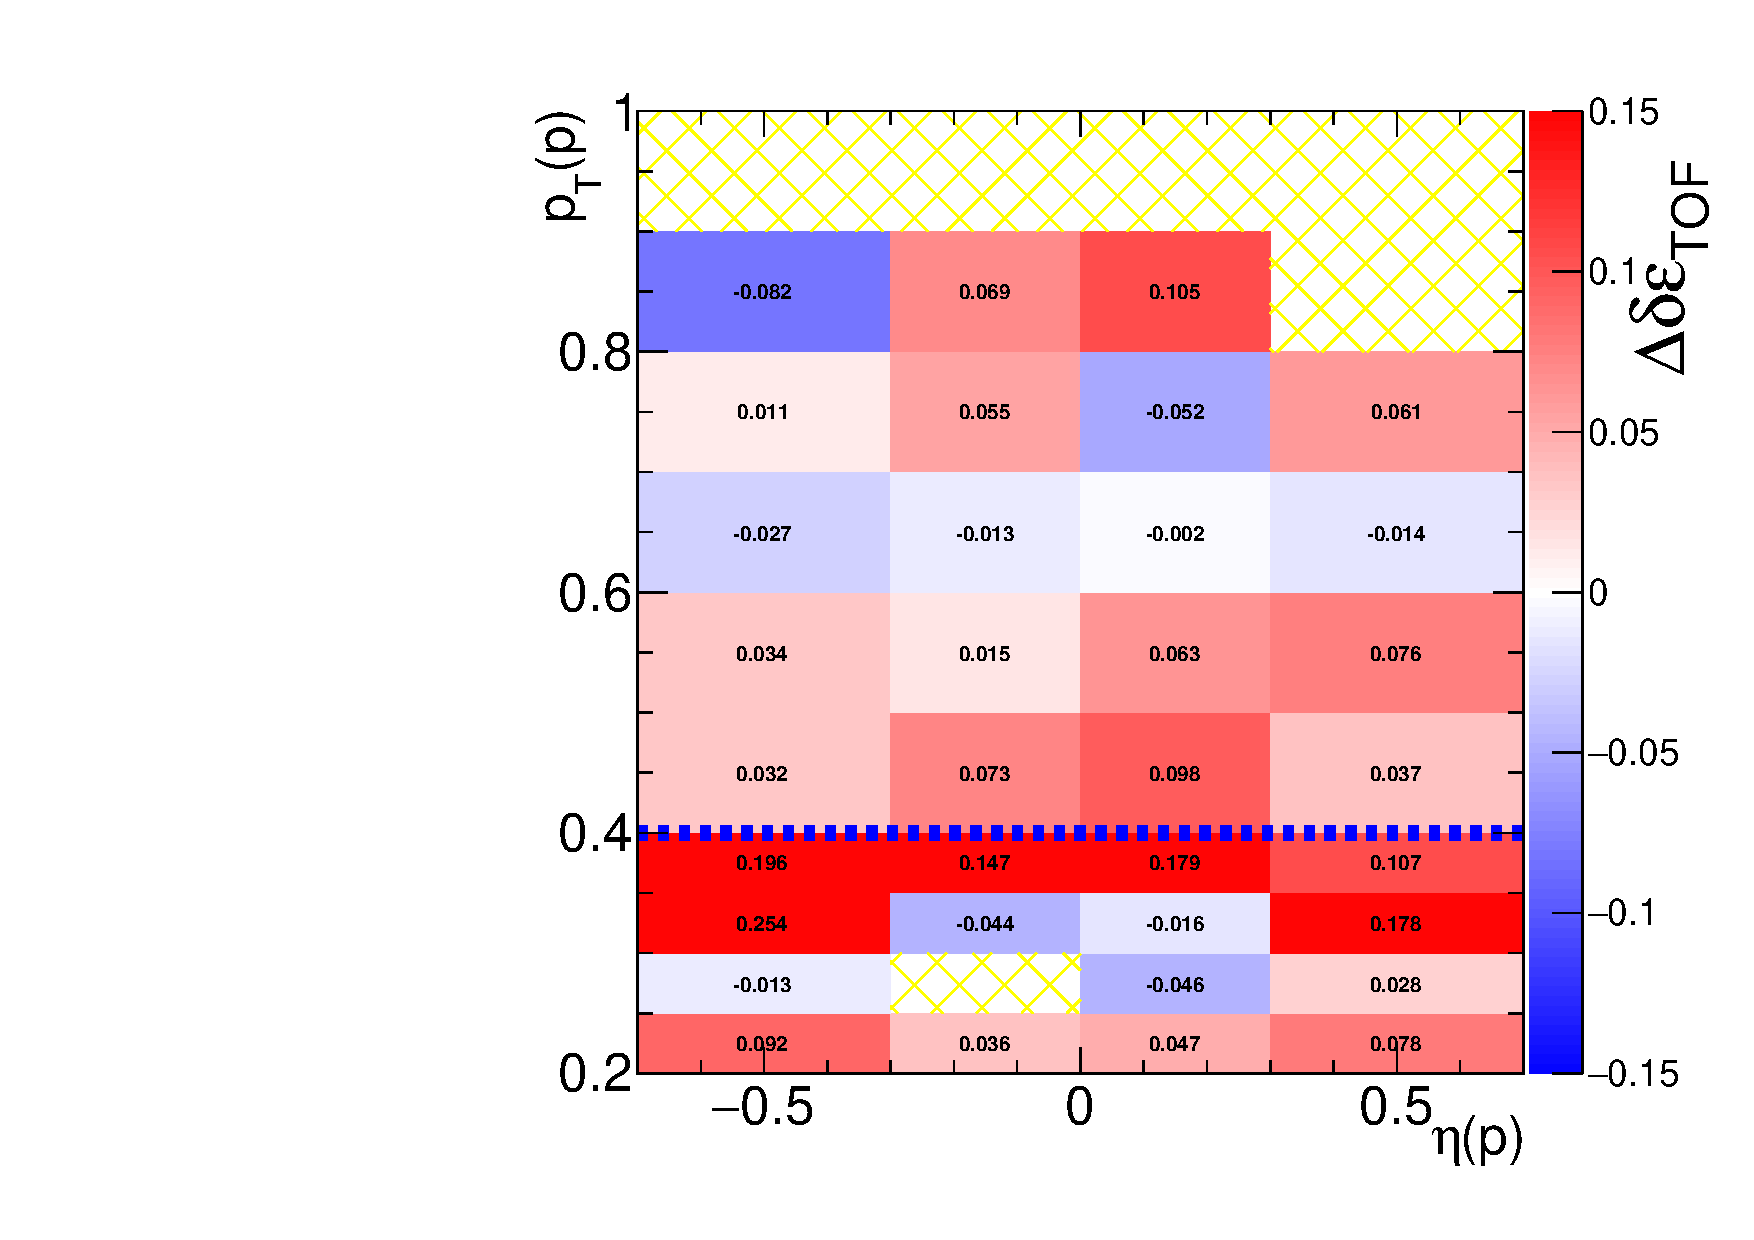
\includegraphics[width=\linewidth]{graphics/systematicsEfficiency/TofSyst/tofEffDifference_Delta_proton.pdf}\vspace{-12pt}}}
  \end{subfigure}
}
\caption[Difference between the TOF eff. correction estimated with tag\&probe method and with the HFT-tagged tracks.]%
    {Difference between the TOF eff. correction estimated with tag\&probe method on CEP $\pi^{+}\pi^{-}$ events and with the HFT-tagged tracks for pions (\ref{fig:tofEffDifference_Delta_pion}), kaons (\ref{fig:tofEffDifference_Delta_kaon}) and protons (\ref{fig:tofEffDifference_Delta_proton}). Figure \ref{fig:tofEffDifference_Delta_pion} is the difference between \ref{fig:tofEffDifference_pion} and \ref{fig:TPcorrectionTofEff2D}, Figure \ref{fig:tofEffDifference_Delta_kaon} is the difference between \ref{fig:tofEffDifference_kaon} and \ref{fig:TPcorrectionTofEff2D}, and Figure \ref{fig:tofEffDifference_Delta_proton} is the difference between \ref{fig:tofEffDifference_proton} and \ref{fig:TPcorrectionTofEff2D}. Yellow hatched area mark bins which were empty in histograms for HFT-tagged tracks (thus difference is incalculable). Dashed horizontal lines represent minimum track $p_{T}$ thresholds used in our analyses: $0.3$~GeV for kaons (green) and $0.4$~GeV for protons (blue).}\label{fig:tofEffDifference_Delta}% 
\end{figure}
%---------------------------



\section{Roman Pot track reconstruction efficiency}\label{sec:rpTrackRecoEffSystematics}

\subsection{Track reconstruction efficiency (absolute reconstruction efficiency)}\label{subsec:rpTrackRecoEffSyst}

Nominally the RP track reconstruction efficiency is calculated with the zero-bias-embedded MC events as a probability that forward scattered proton is transported from the IP to the RP stations and produces hits in SSDs that are reconstructed as a track point(s) that form a track which passes selection cuts. The systematic uncertainty of this efficiency, which reflects the accuracy of the simulation (modeling of the dead material, signal digitization etc.), has been estimated using elastic scattering events. The same analysis scheme was used for the data and for embedded elastic scattering MC events. The difference between efficiency estimates extracted from the data and simulation was established as a measure of the systematic uncertainty of the nominal RP track reconstruction efficiency.

An idea of this analysis was to select elastic proton-proton scattering events by requiring the elastic trigger (signal in PMTs in two opposite RP branches) and clean RP track of $\xi=0$ on one side of the IP, and counting how often there is reconstructed and successfully selected collinear RP track in the opposite branch with trigger signal. The method is illustrated in Fig.~\ref{fig:sketchRpTrackEffSyst}. Detailed description of the algorithm is provided below:
\begin{enumerate}
\item RP\_ET triggers were used. Elastic proton-proton scattering MC events (generated with $B=14.3~\text{GeV}^{-2}$ as it was measured in independent analysis, see Ref.~\cite{ElasticNote}) simulated in Geant4 and embedded into zero-bias data were subjected to the same trigger conditions (signal in trigger counters in opposite RP branches was required). The zero-bias data used in embedding was taken from the same runs for which RP\_ET triggers were analyzed. Also number of simulated events for each run was proportional to number of elastic scattering events in given run.\vspace{-4pt}
\item Since RP\_ET triggers can be fired not only by elastic interactions but also, for instance, by central diffraction events, minimum bias events with forward remnants of protons, overlap of single diffraction events with beam halo protons, etc., a list of vetoes was exerted to suppress non-elastic interaction/pile-up:\vspace*{-7pt}
\begin{multicols}{3}
	\begin{itemize}
		\item TOF L0 mulitplicity = 0
		\item n. of TPC-TOF tracks = 0
		\item n. of recon. TOF hits = 0
		\item empty ZDC
		\item empty VPD
		\item empty BBC (small, large)
		\item false state of RP\_IT trigger bit (trigger signal only in RP branches forming an elastic trigger bit RP\_ET)
	\end{itemize}
\end{multicols}\vspace{-10pt}
As shown in Fig.~\ref{fig:rpSystXi_EU}, the mentioned types of background events that fire RP\_ET trigger are vastly suppressed with the above vetoes.\vspace{-4pt}
\item From the difference between average time of the trigger signal in west and east RPs the $z$-position of the vertex was reconstructed and required to satisfy condition $|z_{\text{vtx}}|<80$~cm, which is the same as the range of $z_{\text{vtx}}$ accepted in our physics analyses.\vspace{-4pt}
\item One side (a 'tagging' side, or a reference side) was checked if a clean set of track points was reconstructed in a branch with trigger signal. By clean set of track points we understand either 1 and 0, 0 and 1, or 1 and 1 reconstructed track point in the $1^{\text{st}}$ and $2^{\text{nd}}$ RP in given branch, respectively. If yes, from this(ese) track point(s) a RP track was formed, reconstructed with the $z$-position of the vertex assumed to be as it was reconstructed in \#3.\vspace{-4pt}
\item Checked if in the 'probed' branch (that has a trigger signal, opposite to the reference branch) there is RP track which passes the track selection used in CEP analysis, and there is exactly 1 such track (as in CEP analysis):\vspace*{-4pt}% (criteria \textbf{C4} in Ref.~\cite{AnalysisNoteRafal}).
\begin{itemize}
  \itemm RP track contains only track-points with at least 3 (out of maximum 4) planes used in reconstrucion,
  \itemm Local angles are consistent with the forward proton track originating from the IP:\vspace{-5pt}
  \[-2~\text{mrad}<\theta_{x}^{\text{RP}}-x^{\text{RP}}/|z^{\text{RP}}|<4~\text{mrad},~~~~~-2~\text{mrad}<\theta_{y}^{\text{RP}}-y^{\text{RP}}/|z^{\text{RP}}|<2~\text{mrad}\]
\end{itemize}\vspace{-4pt}
If the above was satisfied, the collinearity was calculated between the track reconstructed in the branch under study and the reference track (Fig.~\ref{fig:rpSystCollinearity}). If the collinearity was within 3.5 standard deviations the elastic track was claimed reconstructed.\vspace{-4pt}
\item The RP track reconstruction efficiency $\varepsilon$ was defined as a probability that in the studied branch exactly 1 RP track was reconstructed and selected, and found collinear with the reference track within 3.5 standard deviations (as required in \#5). It was calculated as a ratio of the number of events with reconstructed track in a probed branch and clean track in tagging branch, to all number of events with clean track in tagging branch.\vspace{-4pt}
\item Steps \#4-\#6 were repeated for the other side.
\end{enumerate}
The efficiencies obtained with the described method were calculated as a function of the expected transverse momentum components of the proton in the branch under study. These components were assumed to be equal to the $(p_{x},p_{y})$ of the track in the tagging branch taken with the "-" sign to reflect the fact that elastically scattered protons have opposite momentum, $(p_{x}^{\text{E}},p_{y}^{\text{E}},p_{z}^{\text{E}}) = (-p_{x}^{\text{W}},-p_{y}^{\text{W}},-p_{z}^{\text{W}})$ (in the center-of-mass reference frame, which here is identical with the laboratory frame). The sample result for a single branch is presented in Fig.~\ref{fig:totalRpRecoEff_EU}. The remaining results were placed in Appendix~\ref{appendix:rpTrackRecoEffSyst}.

From the figures one can read that the difference between the RP track reconstruction efficiency estimated from the data and from embedded MC do not differ by more than $\sim5\%$, on average by not more than $\sim2\%$. The largest difference between the data and simulation is observed in the corner of the fiducial region where the RF shield is present between the $1^{\text{st}}$ and $2^{\text{nd}}$ RP station. This may indicate that the thickness of this shield is not accurately modeled (too thick piece of material implemented in the simulation). More significant differences are generally observed close to the edges of the fiducial region rather than its center. This could be an influence of the angular beam divergence which was assumed constant in the simulation, while in the data it changes over time (grows with the RHIC store lifetime). However, the scale of the inconsistencies between the data and MC is satisfactorily low hence we accept them as the estimate of the systematic uncertainty of the RP track reconstruction efficiency. The systematic uncertainty assigned to the track of reconstructed $(p_{x}, p_{y})$ is equal to the absolute value of the difference shown in Fig.~\ref{fig:totalRpRecoEff2D_EU} and similar differences in Appendix~\ref{appendix:rpTrackRecoEffSyst}.
\begin{equation}
 0.2<|p_{y}|<0.4,~~~-0.2<p_{x},~~~(p_{x}+0.3)^{2}+p_{y}^{2}<0.5^{2}~~~(\text{all in GeV})
\end{equation}

\begin{figure}[t!]%\vspace{-34pt}
	\centering
	\parbox{0.65\textwidth}{%
		\centering%
		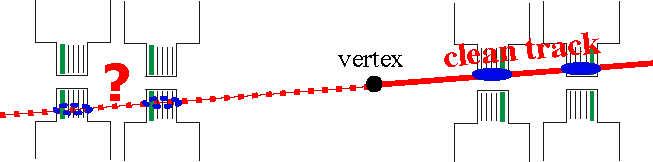
\includegraphics[width=\linewidth]{graphics/systematicsEfficiency/RpSyst/effCalculationScheme.pdf}%
	} 
	\quad
	\parbox{0.31\textwidth}{ 
		\centering
		%\begin{minipage}[t][0.64\linewidth][t]{\linewidth}%\vspace{73pt} 
			\caption[Draft of the method of estimation of the RP track reconstruction efficiency for systematic uncertainty determination.]%
			{Sketch of the Roman Pot system with drafted method of estimation of the RP track reconstruction efficiency using elastic scattering events.}\label{fig:sketchRpTrackEffSyst}% 
		%\end{minipage}
	}
	
\end{figure}
%---------------------------


%---------------------------
\begin{figure}[h]%\vspace{-34pt} 
	\centering
	\parbox{0.4725\textwidth}{%
		\centering%
		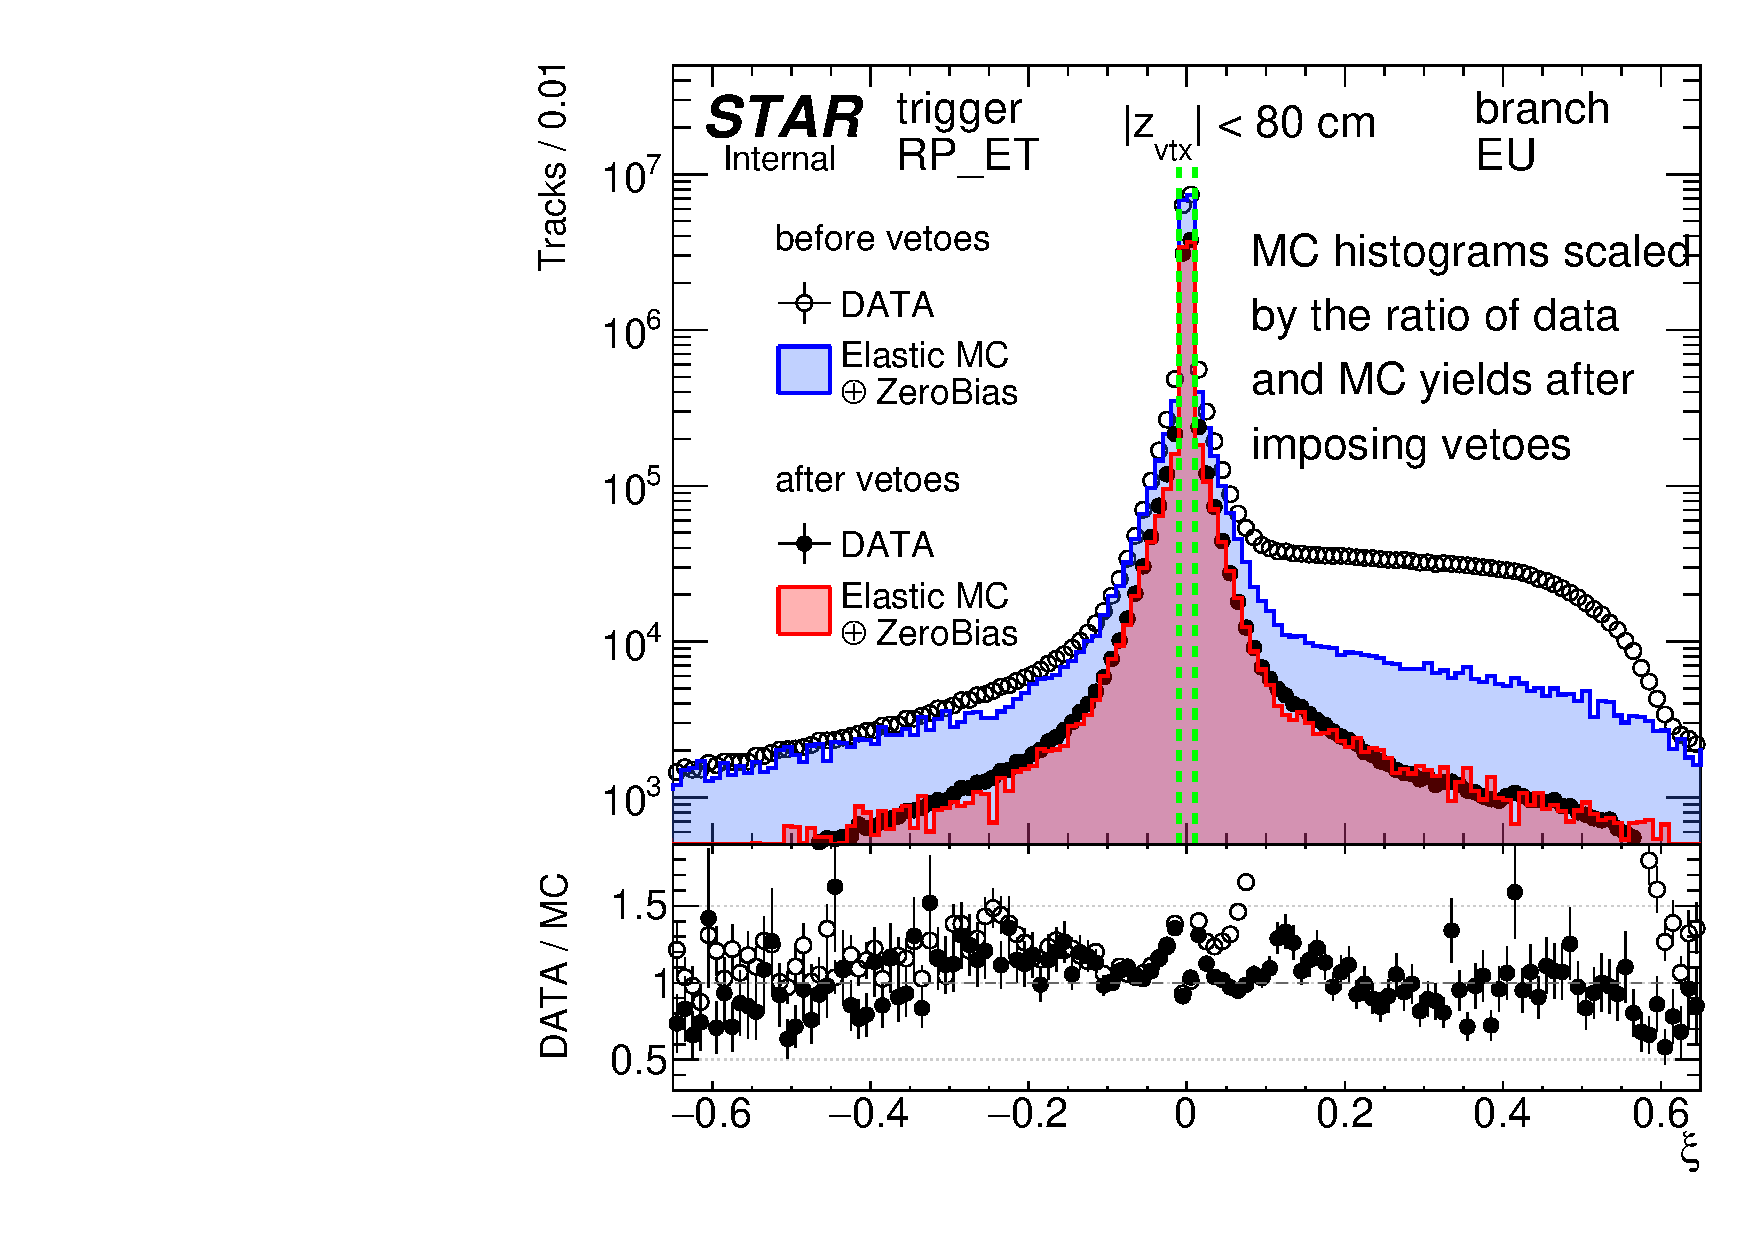
\includegraphics[width=\linewidth,page=1]{graphics/systematicsEfficiency/RpSyst/xiPerBranch.pdf}%
	} 
	\quad
	\parbox{0.4725\textwidth}{ 
		\centering
		%\begin{minipage}[t][0.64\linewidth][t]{\linewidth}%\vspace{73pt} 
			\caption[Fractional momentum loss $\xi$ of clean proton tracks before and after implying vetoes in the data and MC (branch EU).]%
			{Fractional momentum loss $\xi$ of clean proton tracks in branch EU before and after implying vetoes. Data are represented by opened and filled circles, while elastic MC embedded into zero-bias data is drawn as filled histograms. MC histograms are scaled by the ratio of data and MC yields after imposing vetoes in other STAR detector subsystems. Lower pad shows the ratio of corresponding distributions in the data and MC. Before vetoes are applied a significant contribution of non-elastic forward protons in the data sample is clearly visible (excees over MC for $\xi>0.01$). Satisfactory agreement between the data and MC is found after imposing vetoes, which indicates successfull purification of data sample. Dashed green vertical lines show the $\xi$ range of tracks accepted for the RP track (and also track point) efficiency studies, $|\xi|<0.01$. Similar plot for the remaining branches can be found in Appendix~\ref{appendix:rpTrackRecoEffSyst}.}\label{fig:rpSystXi_EU}%  
		%\end{minipage}
	}
	
\end{figure}
%---------------------------


%---------------------------
\begin{figure}[h]
\centering
\parbox{0.4725\textwidth}{
  \centering
  \begin{subfigure}[b]{\linewidth}
                \subcaptionbox{\label{fig:rpSystCollinearity_x}}{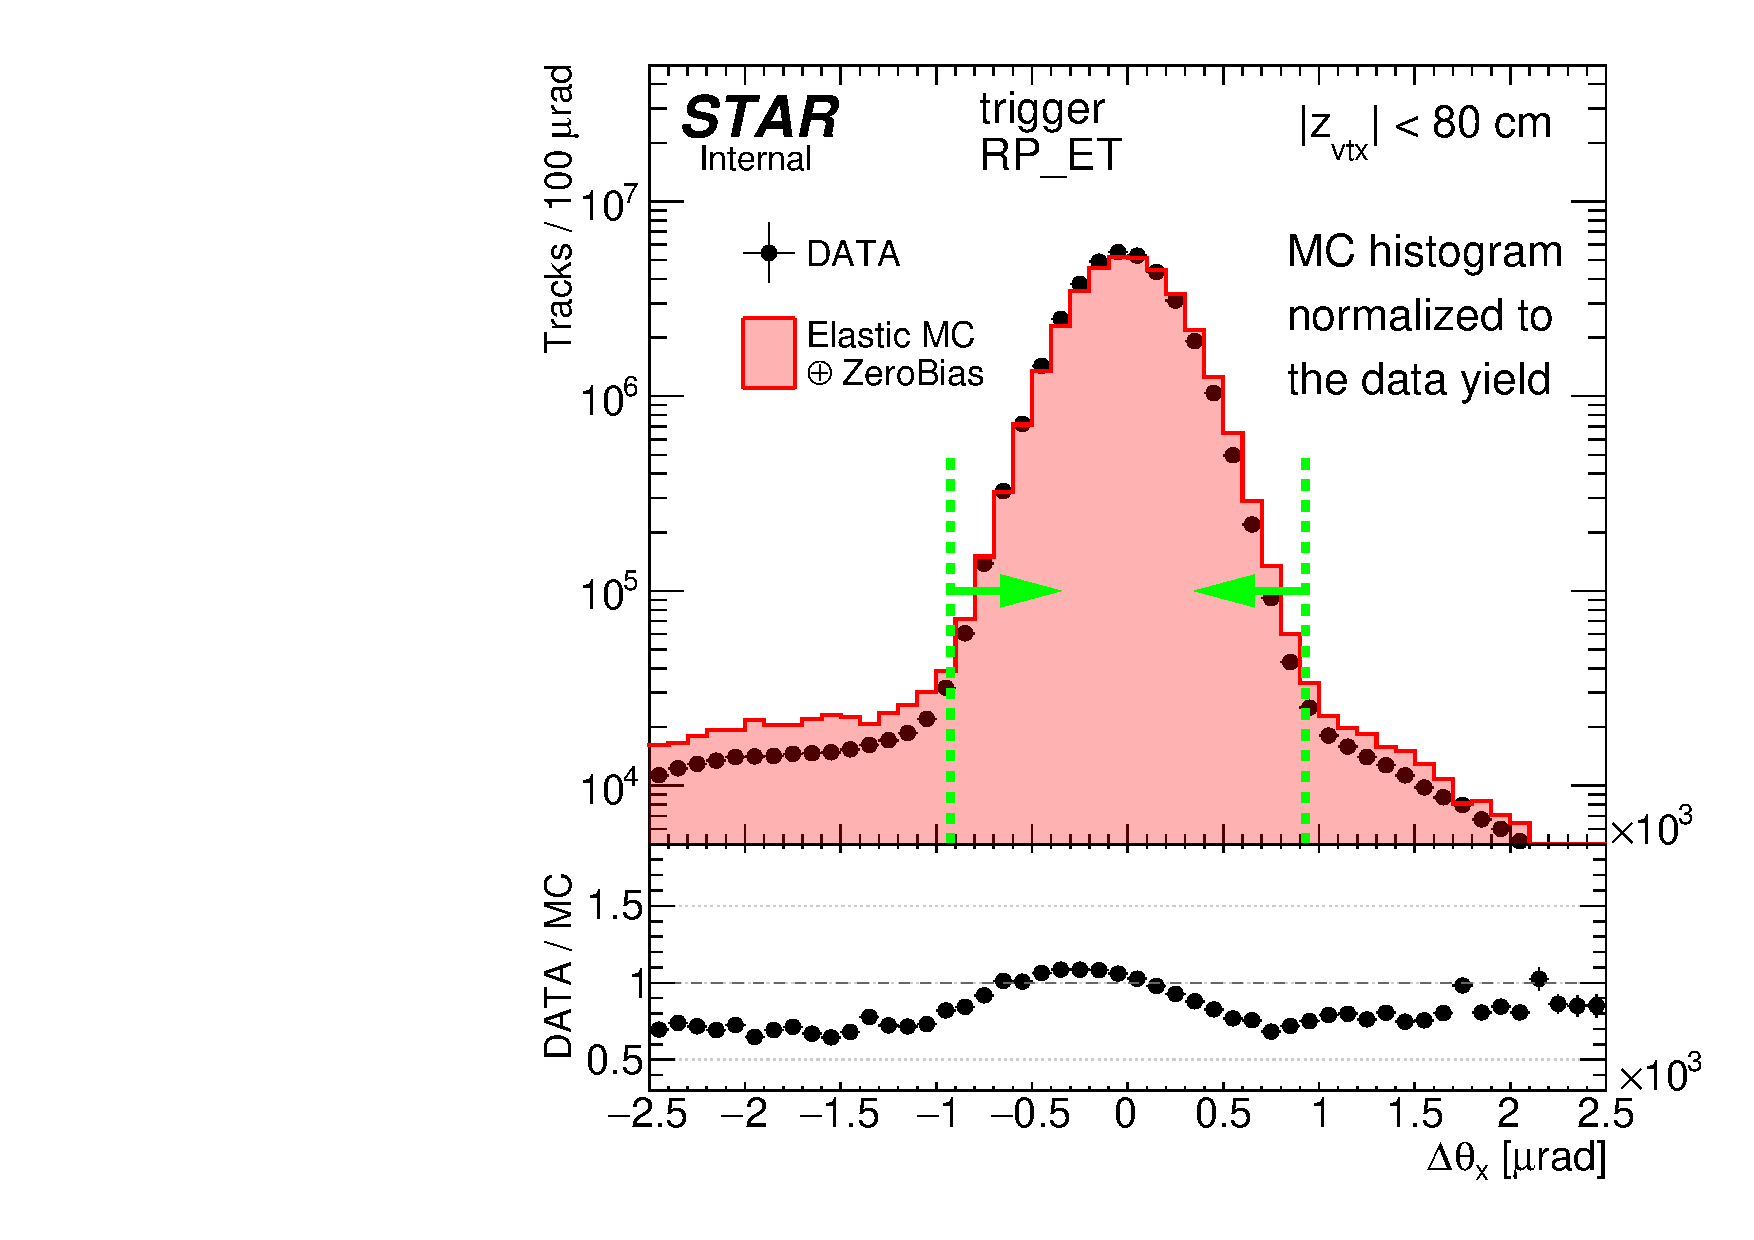
\includegraphics[width=\linewidth,page=1]{graphics/systematicsEfficiency/RpSyst/collinearity.pdf}\vspace{-7pt}}
  \end{subfigure}
}%
\quad\quad%
\parbox{0.4725\textwidth}{
  \centering
  \begin{subfigure}[b]{\linewidth}
                \subcaptionbox{\label{fig:rpSystCollinearity_y}}{\includegraphics[width=\linewidth,page=2]{graphics/systematicsEfficiency/RpSyst/collinearity.pdf}\vspace{-7pt}}
  \end{subfigure}
}%
\caption[Collinearity of a reference track and track reconstructed in studied branch.]%
    {Collinearity of a reference track (the clean track which is required to have $|\xi|<0.1$) and track reconstructed in branch for which reconstruction efficiency is studied. An elastic track is claimed as reconstructed if the collinearity of two tracks does not exceed 3.5 standard deviations, as marked with dashed green vertical lines and arrows.}\label{fig:rpSystCollinearity}%
\end{figure}
%---------------------------

%---------------------------
\begin{figure}[h]%\vspace{-34pt}
	\centering
	\parbox{0.54\textwidth}{
		\centering
		\begin{subfigure}[b]{\linewidth}{\vspace{10pt}
				\subcaptionbox{\label{fig:totalRpRecoEff2D_EU}}{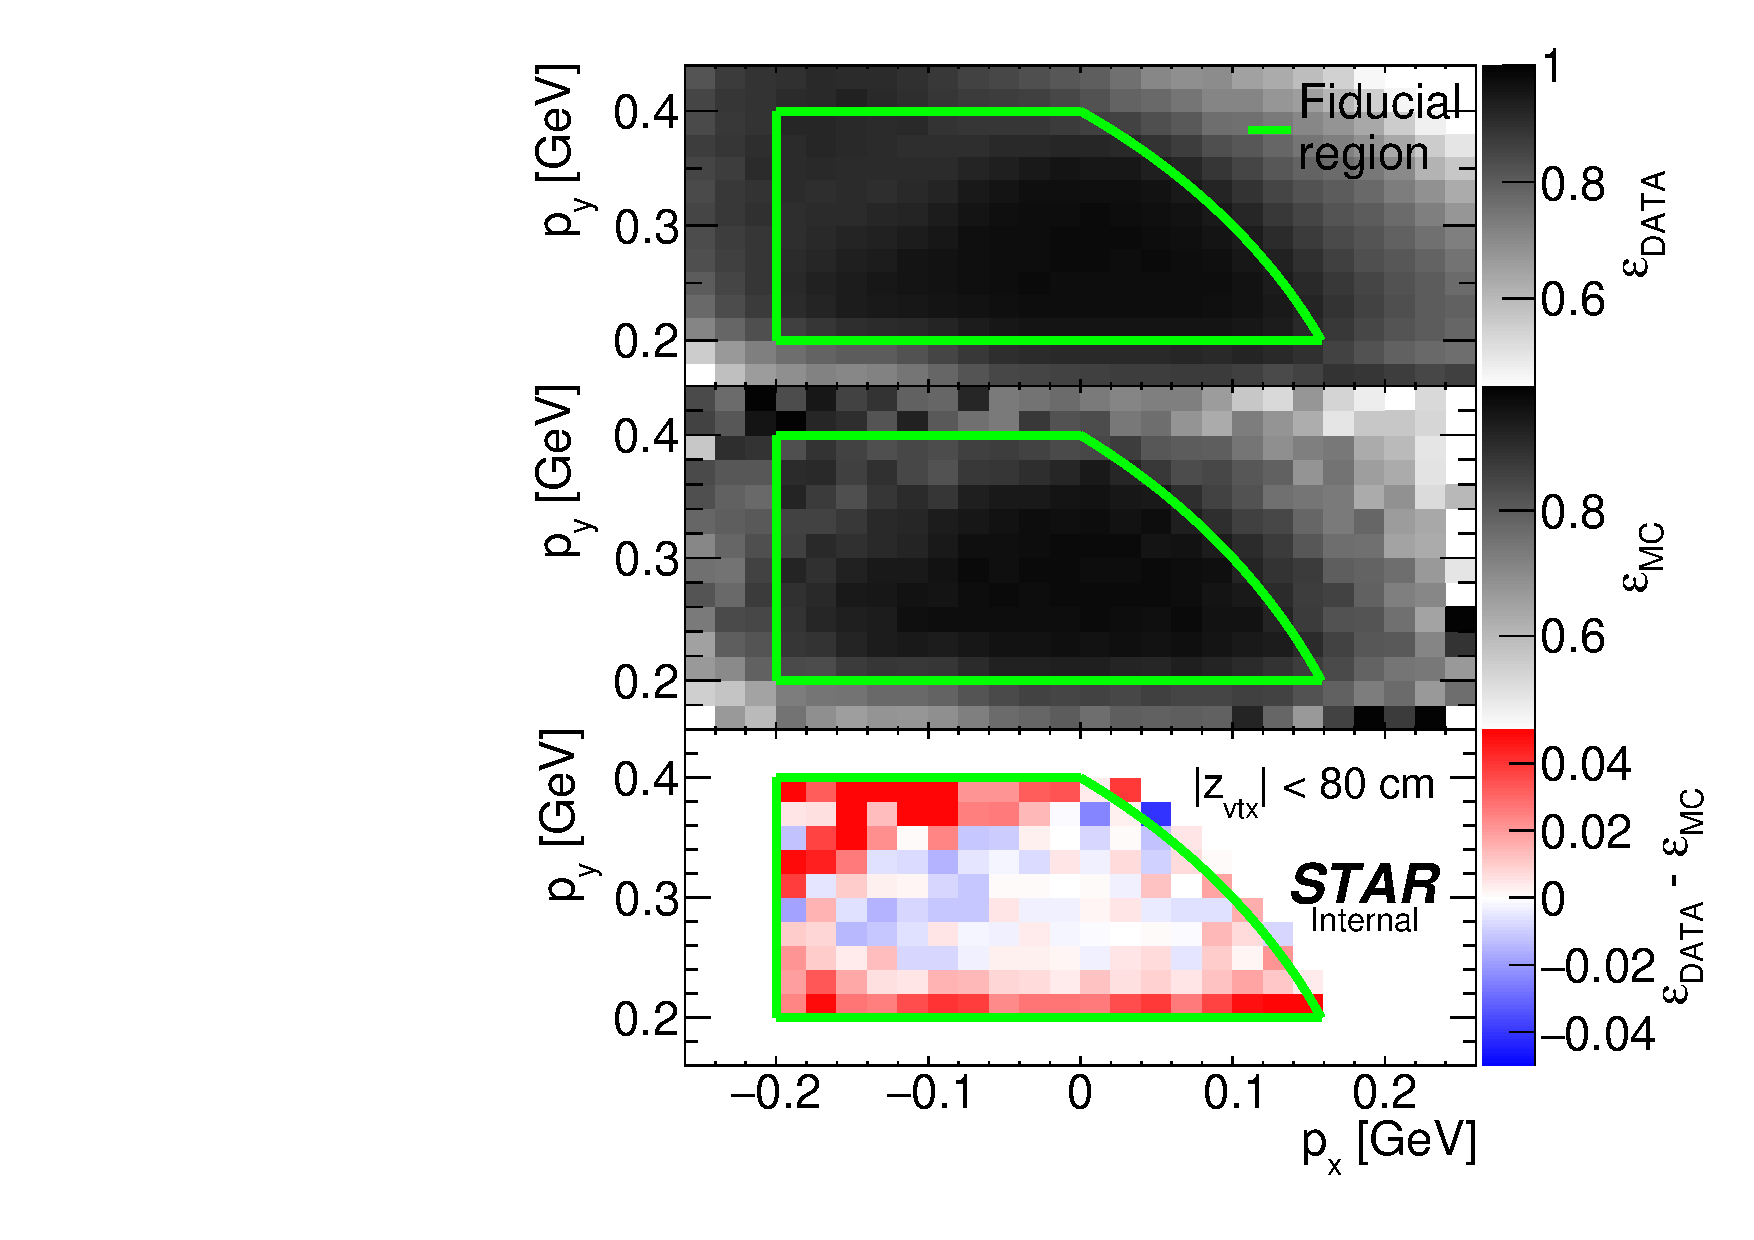
\includegraphics[width=\linewidth,page=1]{graphics/systematicsEfficiency/RpSyst/totalRpRecoEff2D.pdf}\vspace{-12pt}}}
		\end{subfigure}
  \begin{minipage}[t][0.64\linewidth][t]{\linewidth}\vspace{5pt}
	\caption[Coparison of estimated RP track reconstruction efficiency in 2D and 1D (branch EU).]%
	{Sample comparison of RP track reconstruction efficiency (branch EU) estimated with the method described in the text as a function of $(p_{x},p_{y})$ of proton track (\ref{fig:totalRpRecoEff2D_EU}) and comparison of 1-dimensional projections of efficiencies in a fiducial region marked with green envelope: $p_{x}$ (\ref{fig:totalRpRecoEff1D_EU_px}) and $p_{y}$ (\ref{fig:totalRpRecoEff1D_EU_py}). Dashed orange line marks the border between fiducial region part where the correction to RP track reconstruction efficiency is required. Lower pad in each subfigure shows the difference between efficiency extracted from the data and elastic scattering MC embedded into zero-bias data. Hatched orange area marks bins without any entries (efficiency incalculable). The difference between efficiencies in Fig.~'\ref{fig:totalRpRecoEff2D_EU} was calculated only for entries in the fiducial region. Similar plots for the remaining branches can be found in Appendix~\ref{appendix:rpTrackRecoEffSyst}.%
	}\label{fig:totalRpRecoEff_EU}
	\end{minipage}
	%\vspace{14pt}%
	}
	\quad
	\parbox{0.43\textwidth}{
		\centering
		\begin{subfigure}[b]{\linewidth}{
				\subcaptionbox{\label{fig:totalRpRecoEff1D_EU_px}}{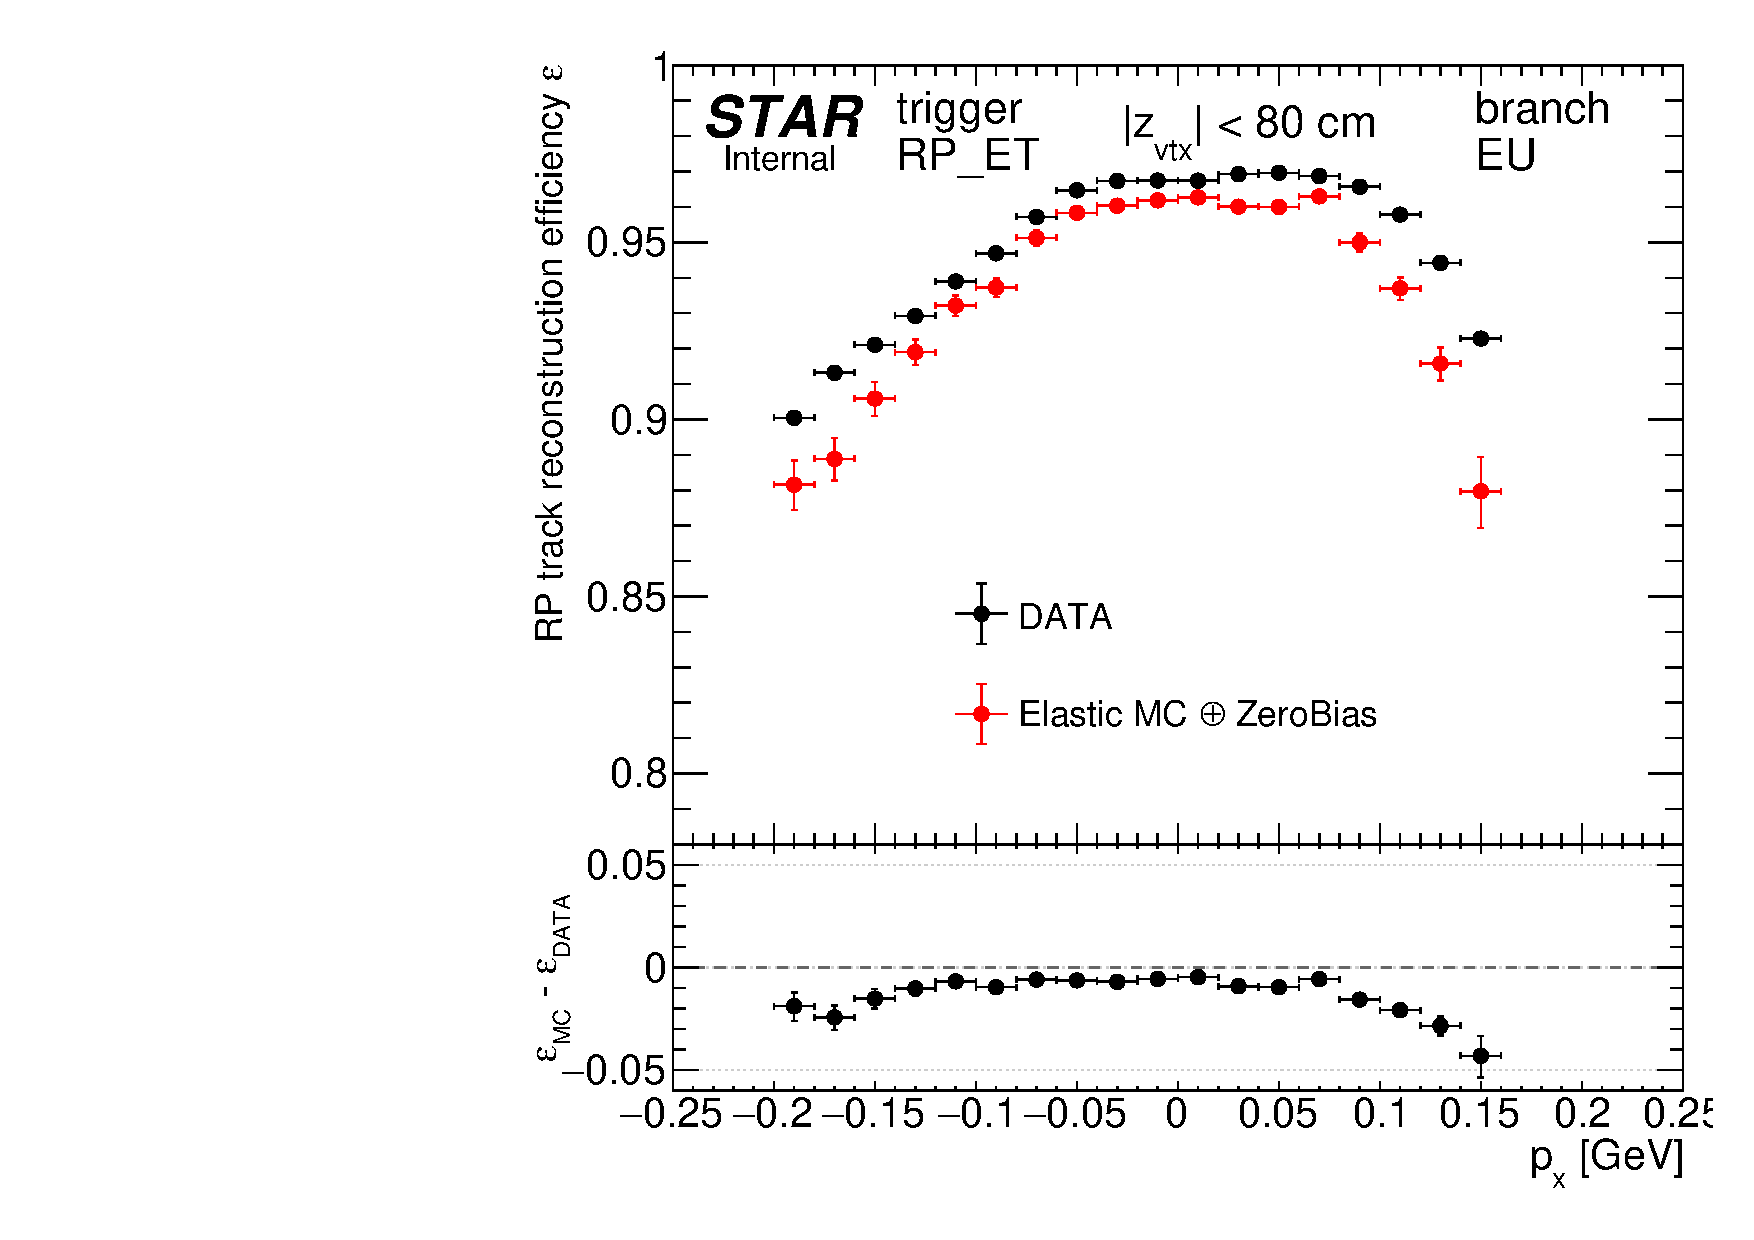
\includegraphics[width=\linewidth,page=1]{graphics/systematicsEfficiency/RpSyst/dataTotalEff_1D.pdf}\vspace{-12pt}}}
		\end{subfigure}
		\begin{subfigure}[b]{\linewidth}{
				\subcaptionbox{\label{fig:totalRpRecoEff1D_EU_py}}{\includegraphics[width=\linewidth,page=2]{graphics/systematicsEfficiency/RpSyst/dataTotalEff_1D.pdf}\vspace{-12pt}}}
		\end{subfigure}
	}
\end{figure}
%---------------------------

\subsection{Track point reconstruction efficiency (relative reconstruction efficiency)}\label{sec:rpTrackPointRecoEffSystematics}

\begin{figure}[h]%\vspace{-34pt}
	\centering
	\parbox{0.65\textwidth}{%
		\centering%
		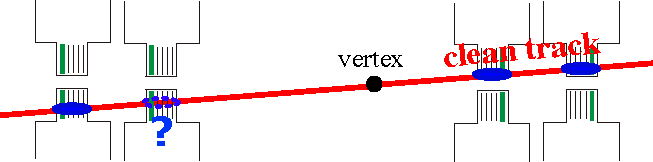
\includegraphics[width=\linewidth]{graphics/systematicsEfficiency/RpSyst/effCalculationScheme_2.pdf}%
	} 
	\quad
	\parbox{0.31\textwidth}{ 
		\centering
		%\begin{minipage}[t][0.64\linewidth][t]{\linewidth}%\vspace{73pt}
			\caption[Draft of the method of estimation of the RP track point reconstruction efficiency for systematic uncertainty determination.]%
			{Sketch of the Roman Pot system with drafted method of estimation of the RP track point reconstruction efficiency using elastic scattering events.}\label{fig:sketchRpTrackPointEffSyst}% 
		%\end{minipage}
	}
	
\end{figure}
%---------------------------





%---------------------------
\begin{figure}[h]
\centering
\parbox{0.4725\textwidth}{
  \centering
  \begin{subfigure}[b]{\linewidth}
                \subcaptionbox{\label{fig:rpSystPositionDifference_x}}{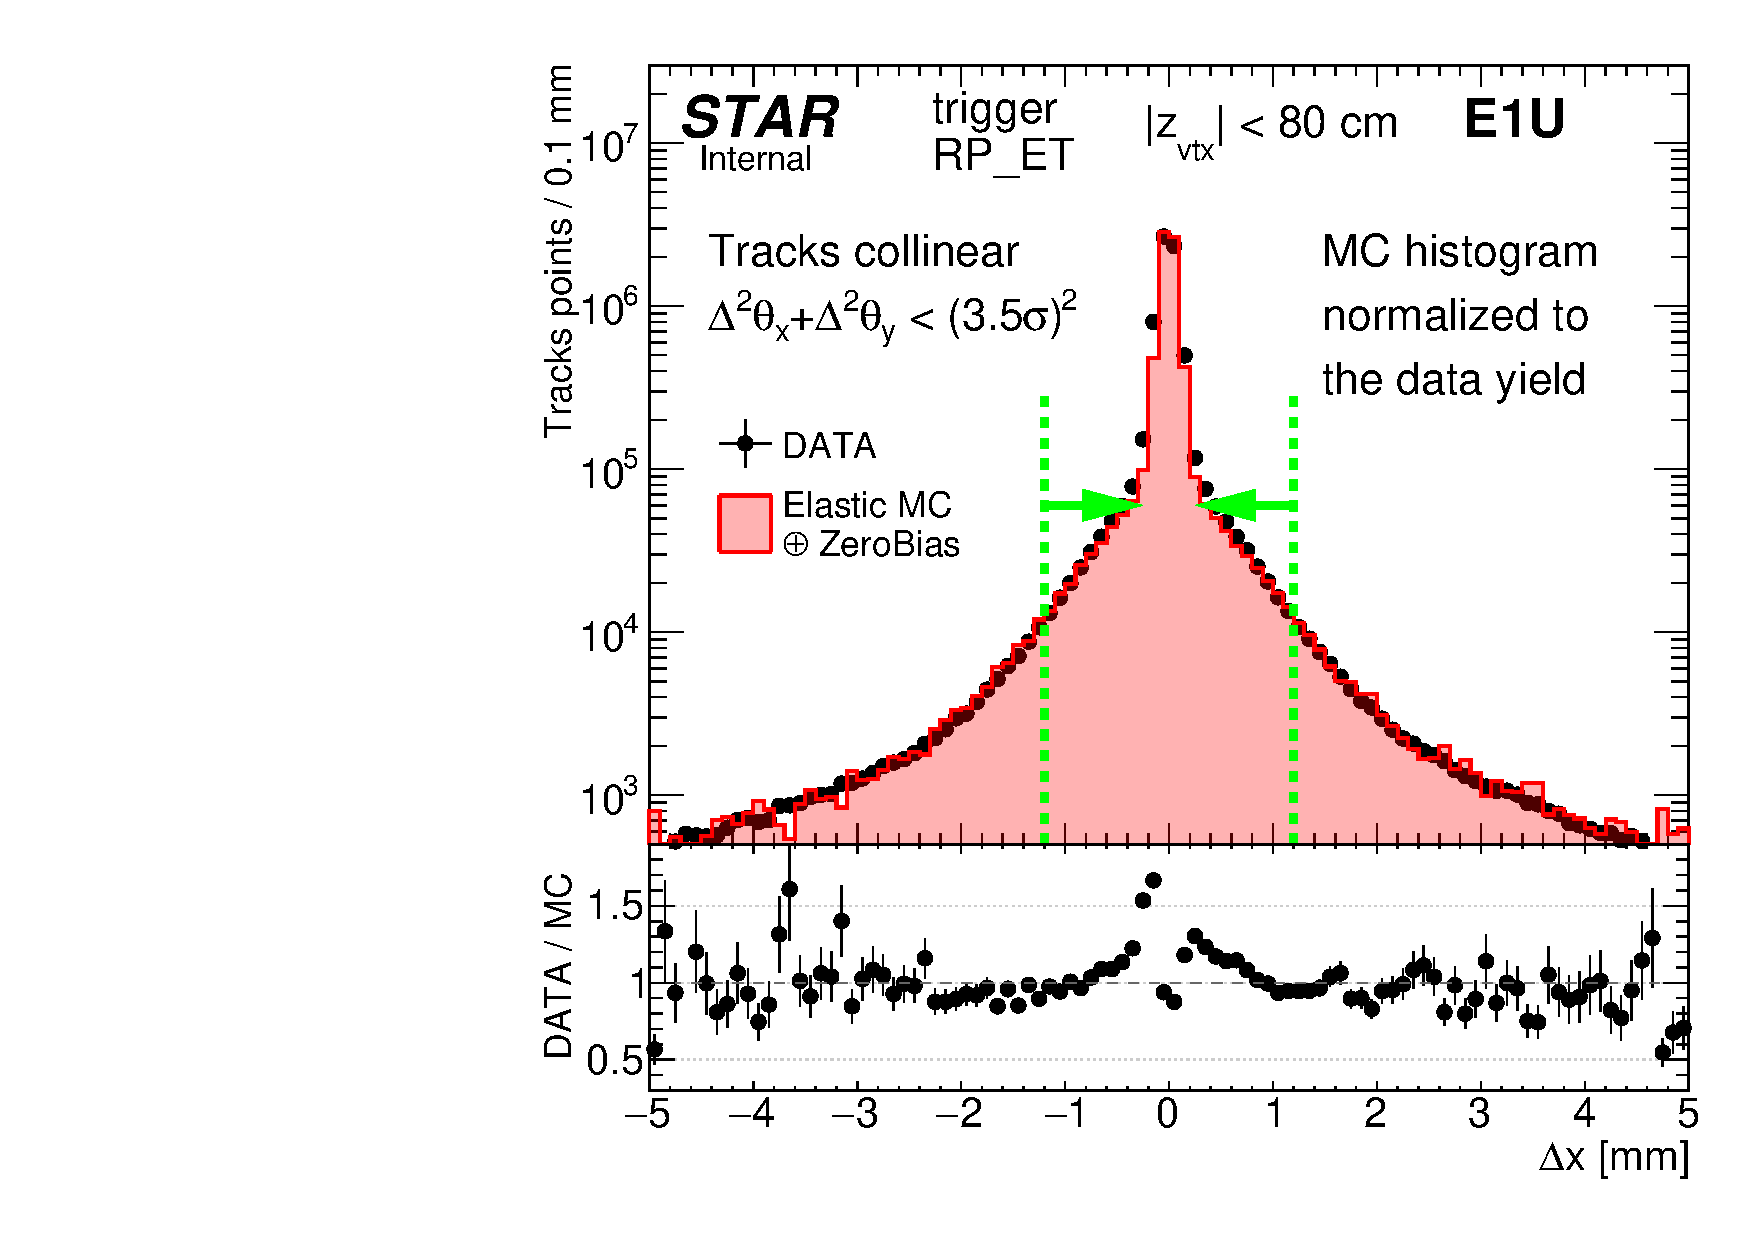
\includegraphics[width=\linewidth,page=1]{graphics/systematicsEfficiency/RpSyst/positionDifference.pdf}\vspace{-7pt}}
  \end{subfigure}
}%
\quad\quad%
\parbox{0.4725\textwidth}{
  \centering
  \begin{subfigure}[b]{\linewidth}
                \subcaptionbox{\label{fig:rpSystPositionDifference_y}}{\includegraphics[width=\linewidth,page=2]{graphics/systematicsEfficiency/RpSyst/positionDifference.pdf}\vspace{-7pt}}
  \end{subfigure}
}%
\caption[Difference between measured and extrapolated position of track point in E1U.]%
    {Difference between position of a track point (with clusters in 3 out 4 silicon planes) reconstructed in E1U (if E1U has a trigger signal) and expected track point position extrapolated from a reference track point reconstructed in E2U, for elastic scattering events with the collinearity of the track in the opposite branch and track reconstructed from a reference track point better than 3.5 standard deviations. A track point is claimed as reconstructed if the position difference is not larger than 1.2~mm, as marked with dashed green vertical lines and arrows.}\label{fig:rpSystPositionDifference}%
\end{figure}
%---------------------------


%---------------------------
\begin{figure}[h]%\vspace{-34pt}  
	\centering
	\parbox{0.4725\textwidth}{
		\centering
		\begin{subfigure}[b]{\linewidth}{%\vspace{10pt}
				\subcaptionbox{\label{fig:relativeRpRecoEff2D_E1U_pxpy}}{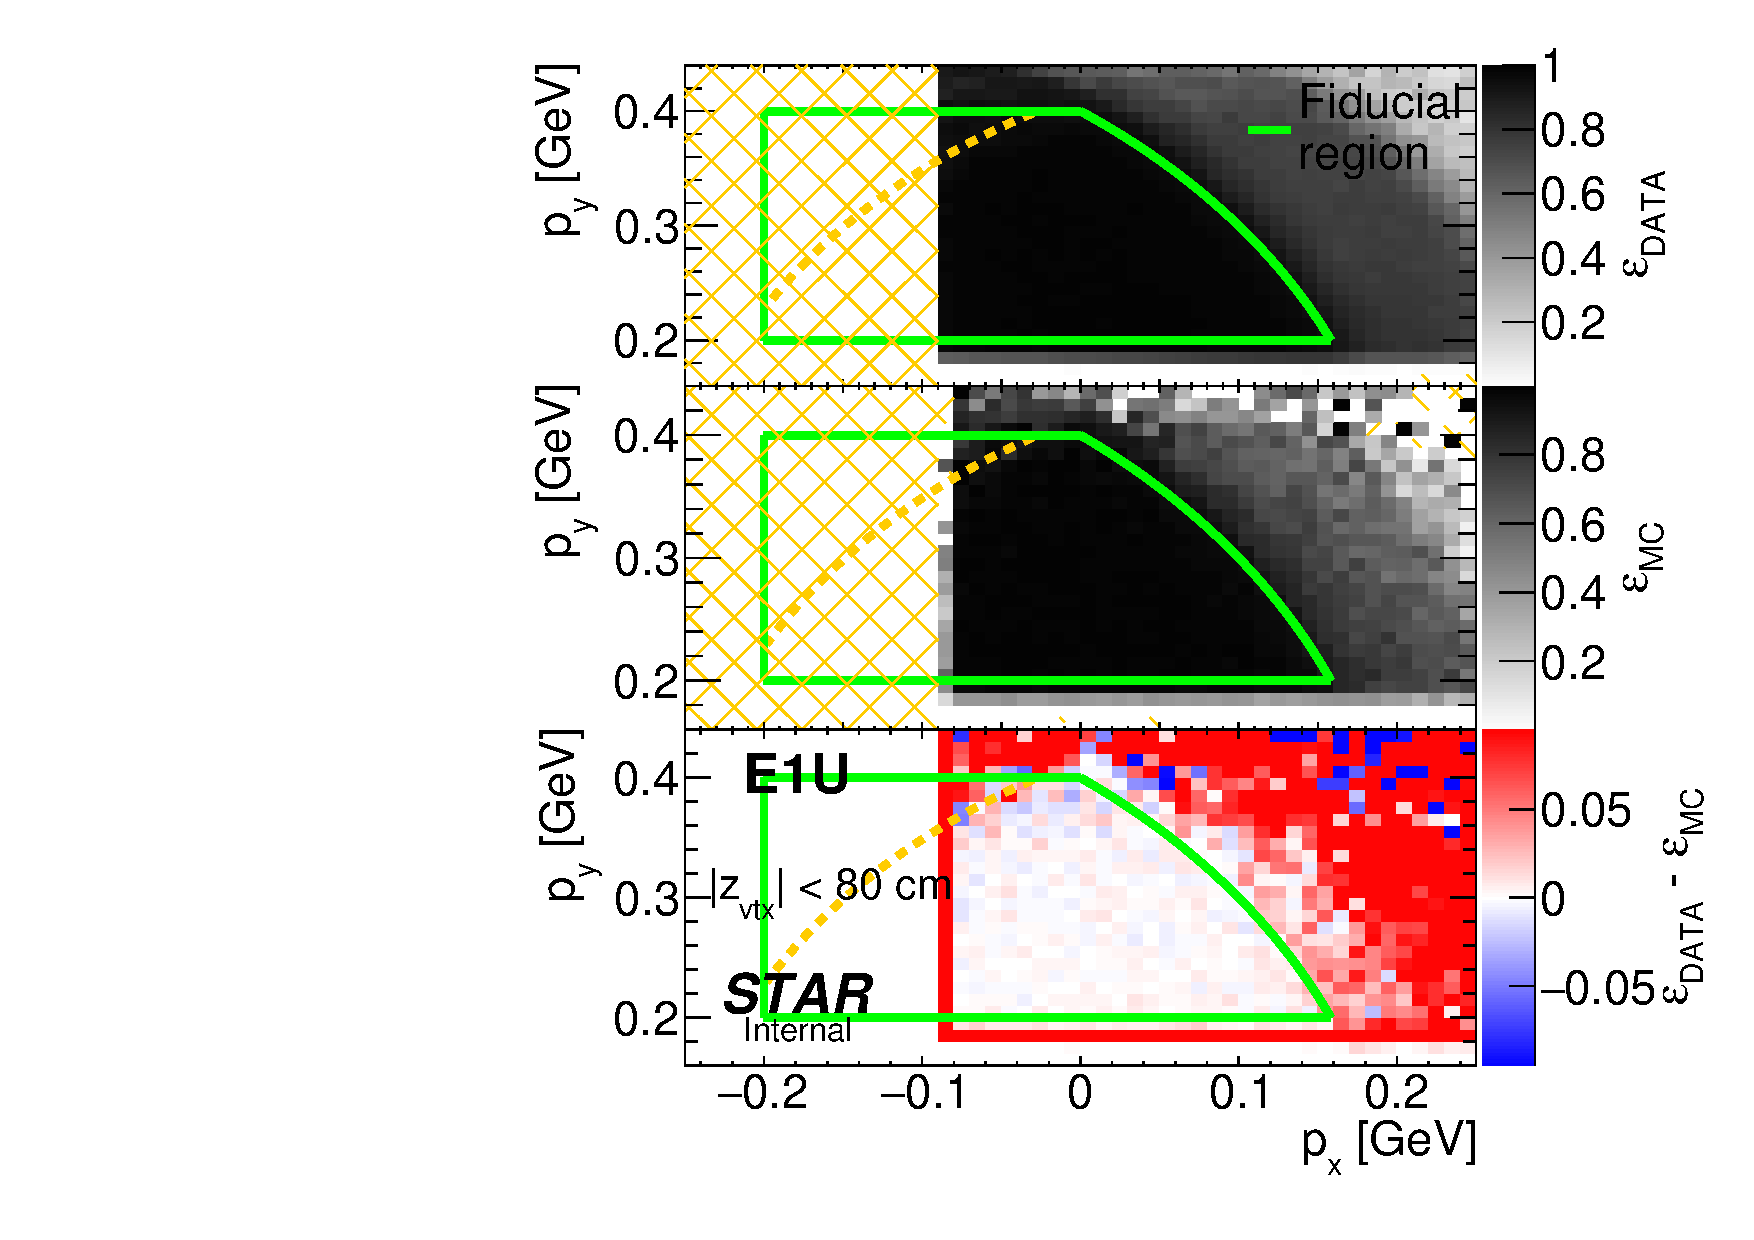
\includegraphics[width=\linewidth,page=1]{graphics/systematicsEfficiency/RpSyst/relativeRpRecoEff2D_pxpy.pdf}\vspace{-12pt}}}
		\end{subfigure}
		\begin{subfigure}[b]{\linewidth}{\addtocounter{subfigure}{1}{
				\subcaptionbox{\label{fig:relativeRpRecoEff1D_E1U_x}}{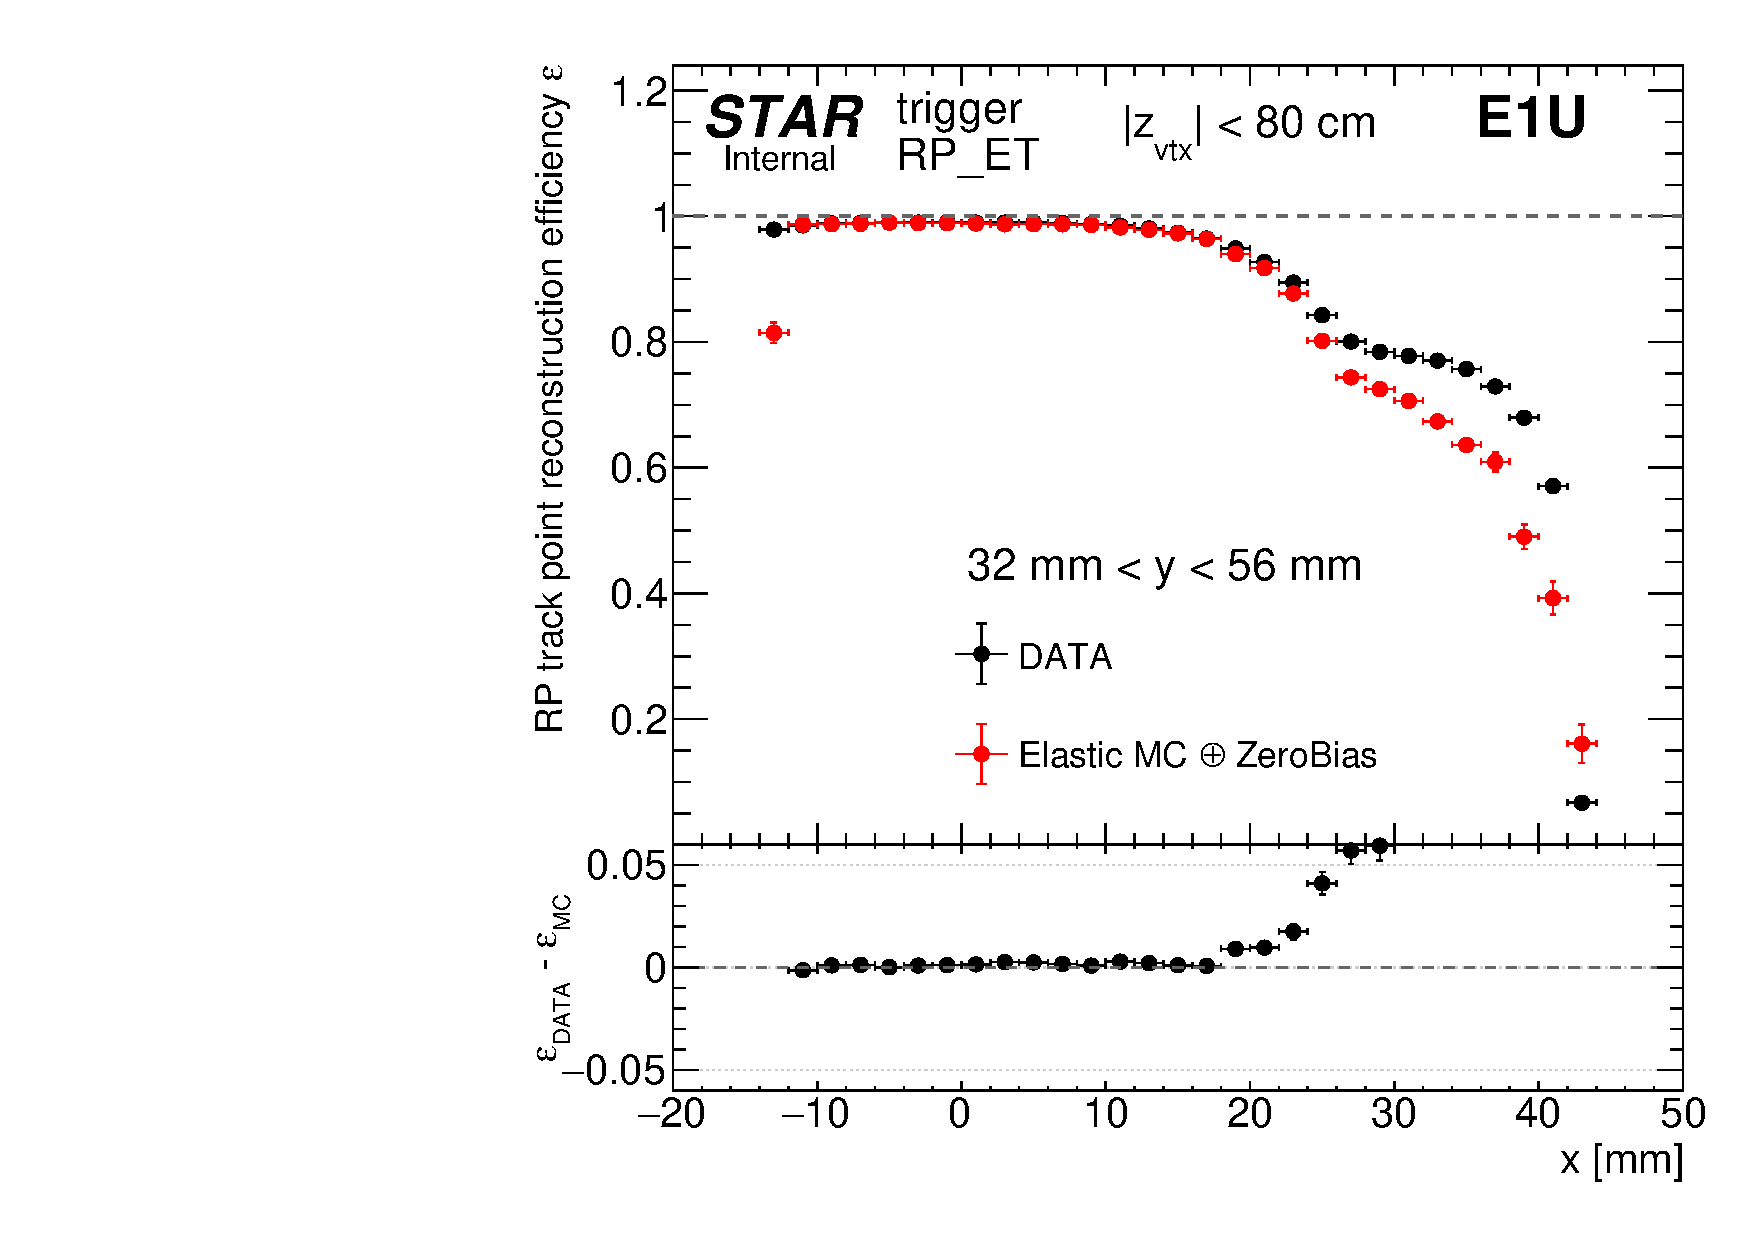
\includegraphics[width=\linewidth,page=1]{graphics/systematicsEfficiency/RpSyst/dataRelativeEff_1D.pdf}\vspace{-12pt}}}}
		\end{subfigure}
	}
	\quad
	\parbox{0.4725\textwidth}{
		\centering
		\begin{subfigure}[b]{\linewidth}{\addtocounter{subfigure}{-2}{%\vspace{10pt} 
				\subcaptionbox{\label{fig:relativeRpRecoEff2D_E1U_xy}}{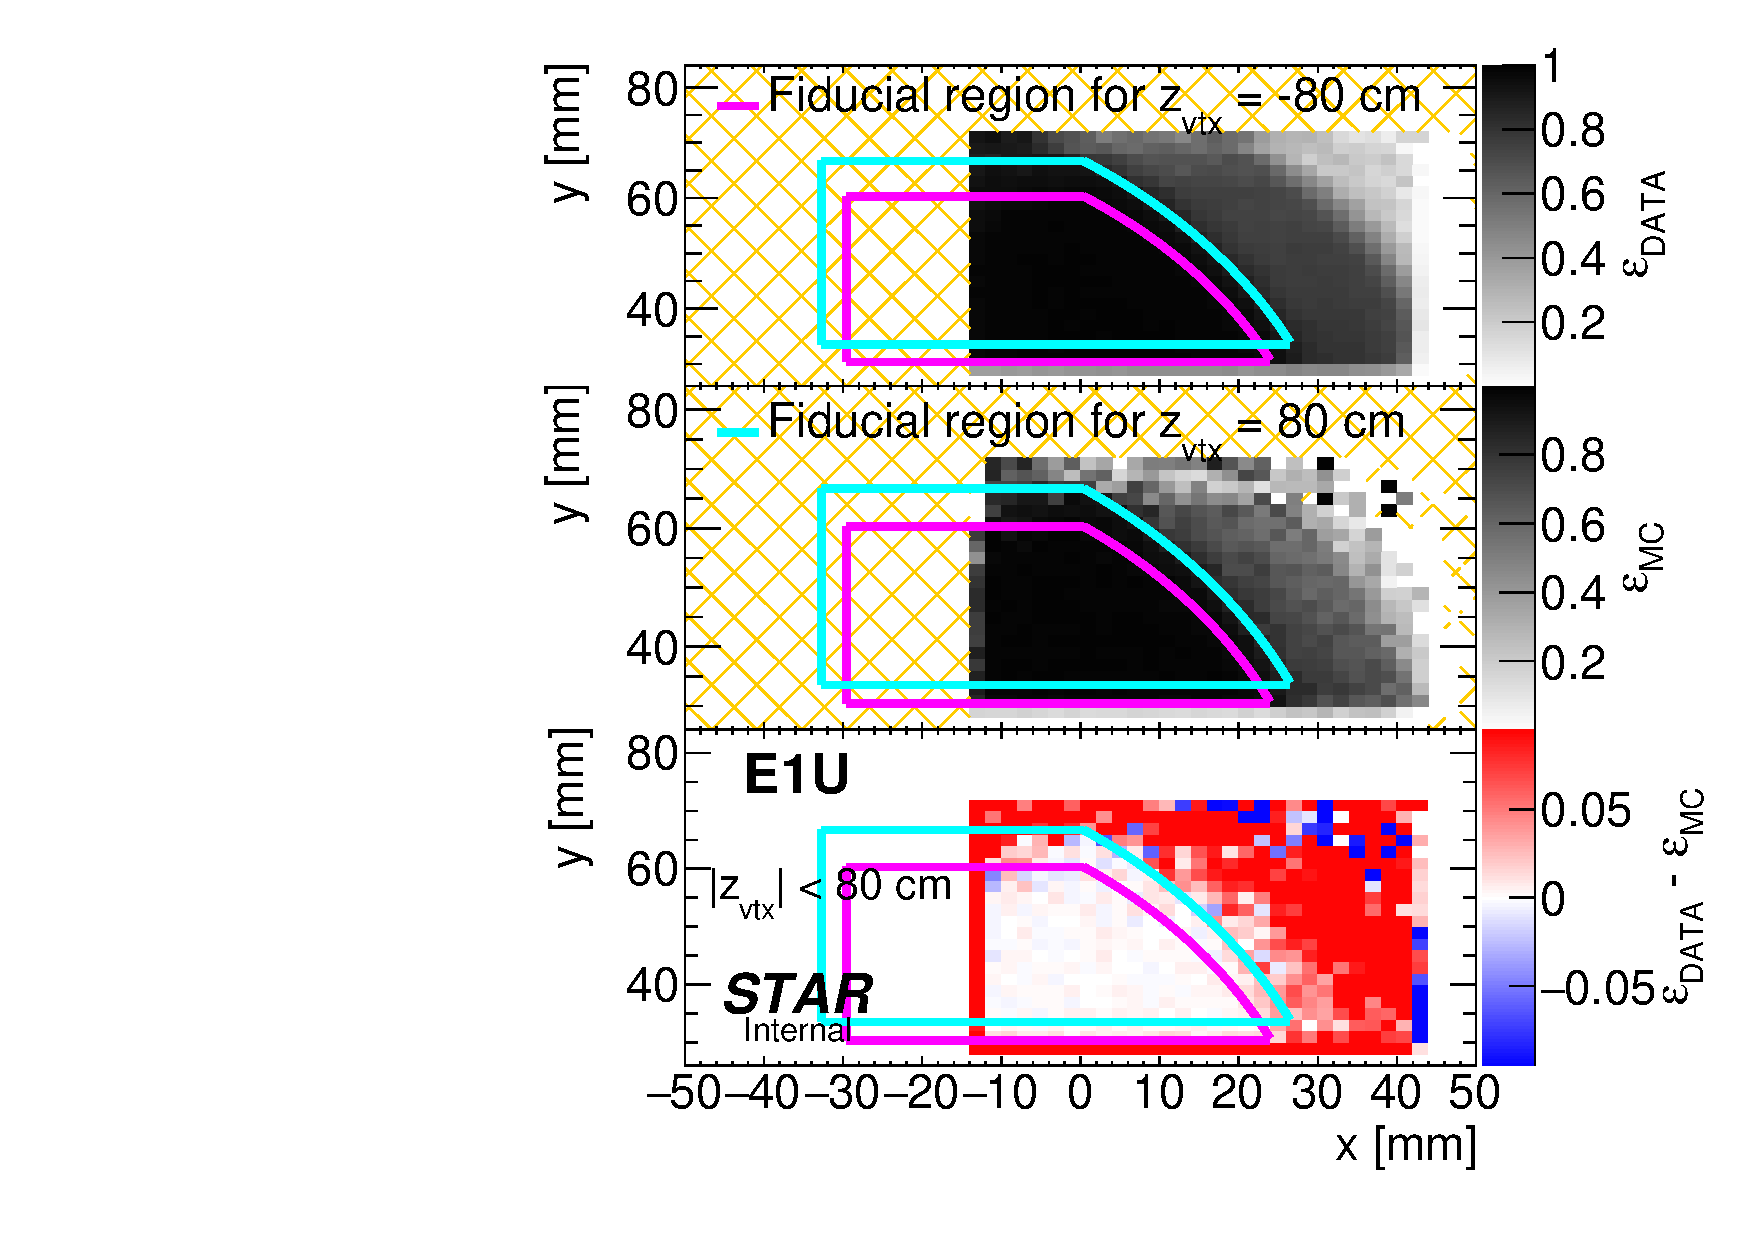
\includegraphics[width=\linewidth,page=1]{graphics/systematicsEfficiency/RpSyst/relativeRpRecoEff2D.pdf}\vspace{-12pt}}}}
		\end{subfigure}
		\begin{subfigure}[b]{\linewidth}{\addtocounter{subfigure}{1}{
				\subcaptionbox{\label{fig:relativeRpRecoEff1D_E1U_y}}{\includegraphics[width=\linewidth,page=2]{graphics/systematicsEfficiency/RpSyst/dataRelativeEff_1D.pdf}\vspace{-12pt}}}}
		\end{subfigure}
	}
	\caption[Coparison of estimated RP track point reconstruction efficiency in 2D and 1D (detector E1U).]%
	{Sample comparison of RP track point reconstruction efficiency (detector E1U) estimated with the method described in the text as a function of $(p_{x},p_{y})$ of proton track (\ref{fig:relativeRpRecoEff2D_E1U_pxpy}), $(x,y)$ position extrapolated from the reference RP (E2U) to the studied RP (\ref{fig:relativeRpRecoEff2D_E1U_xy}), and comparison of 1-dimensional projections of efficiencies in selected ranges of hit position (given in the plot): $x$ (\ref{fig:relativeRpRecoEff1D_E1U_x}) and $y$ (\ref{fig:relativeRpRecoEff1D_E1U_y}). Lower pad in each subfigure shows the difference between efficiency extracted from the data and elastic scattering MC embedded into zero-bias data. Hatched orange area marks bins without any entries (efficiency incalculable). The fiducial region in $(x,y)$ plot is represented by two envelopes which correspond to the extreme accepted values of $z_{vtx}$. Similar plots for the remaining detectors can be found in Appendix~\ref{appendix:rpTrackRecoEffSyst}.% 
	}\label{fig:relativeRpRecoEff_E1U}
\end{figure}
%---------------------------
